\section{Einleitung}

\begin{frame}{Motivation -- Zur Person}
  \begin{columns}
	\begin{column}{0.4\textwidth}
		\begin{itemize}[label=\textcolor{tertiary}{\faicon{caret-right}}]
			\item Kletterer seit 20 Jahren
			\item Jugendleiter für Sportklettern
			\item mehrere eigene Forschungsprojekte
		\end{itemize}
	\end{column}
	\begin{column}{0.5\textwidth}
		\begin{center}
			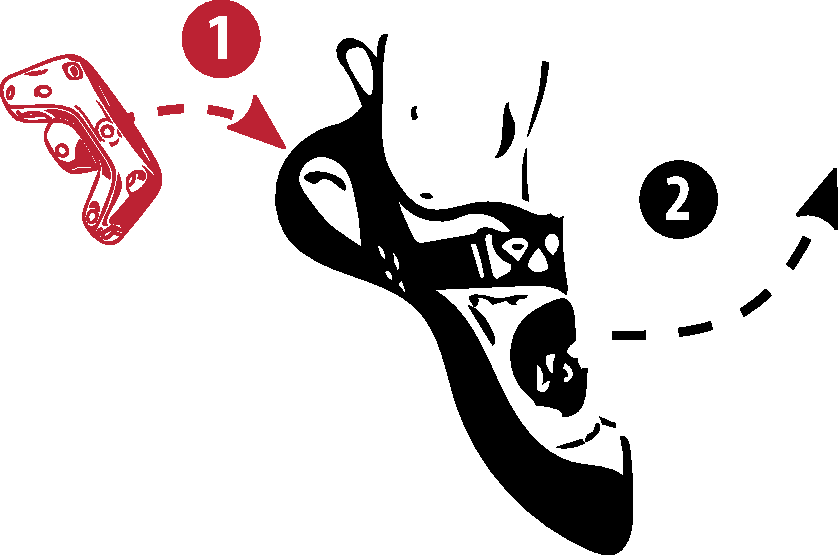
\includegraphics[width=0.8\columnwidth]{include/images/climbing-shoe-with-instructions-on.pdf}
		\end{center}
	\end{column}
\end{columns}
\end{frame}

\begin{frame}{Eigene Forschungsprojekte -- Imagery in Sport Climbing}
\begin{figure}[h]
	\centering
	\begin{subfigure}[t]{0.49\columnwidth}
		\centering
		\begin{overpic}[width=\textwidth]{include/images/Google-Glass.jpg}
			\rbox{-1}{1}{\textcolor{source}{\tiny{Quelle: \href{https://de.wikipedia.org/wiki/Datei:Google_Glass_Main.jpg}{Wikipedia}}}}
		\end{overpic}
		\label{fig:google-glass}
	\end{subfigure}
	\hspace*{\fill}
	\begin{subfigure}[t]{0.49\columnwidth}
		\centering
		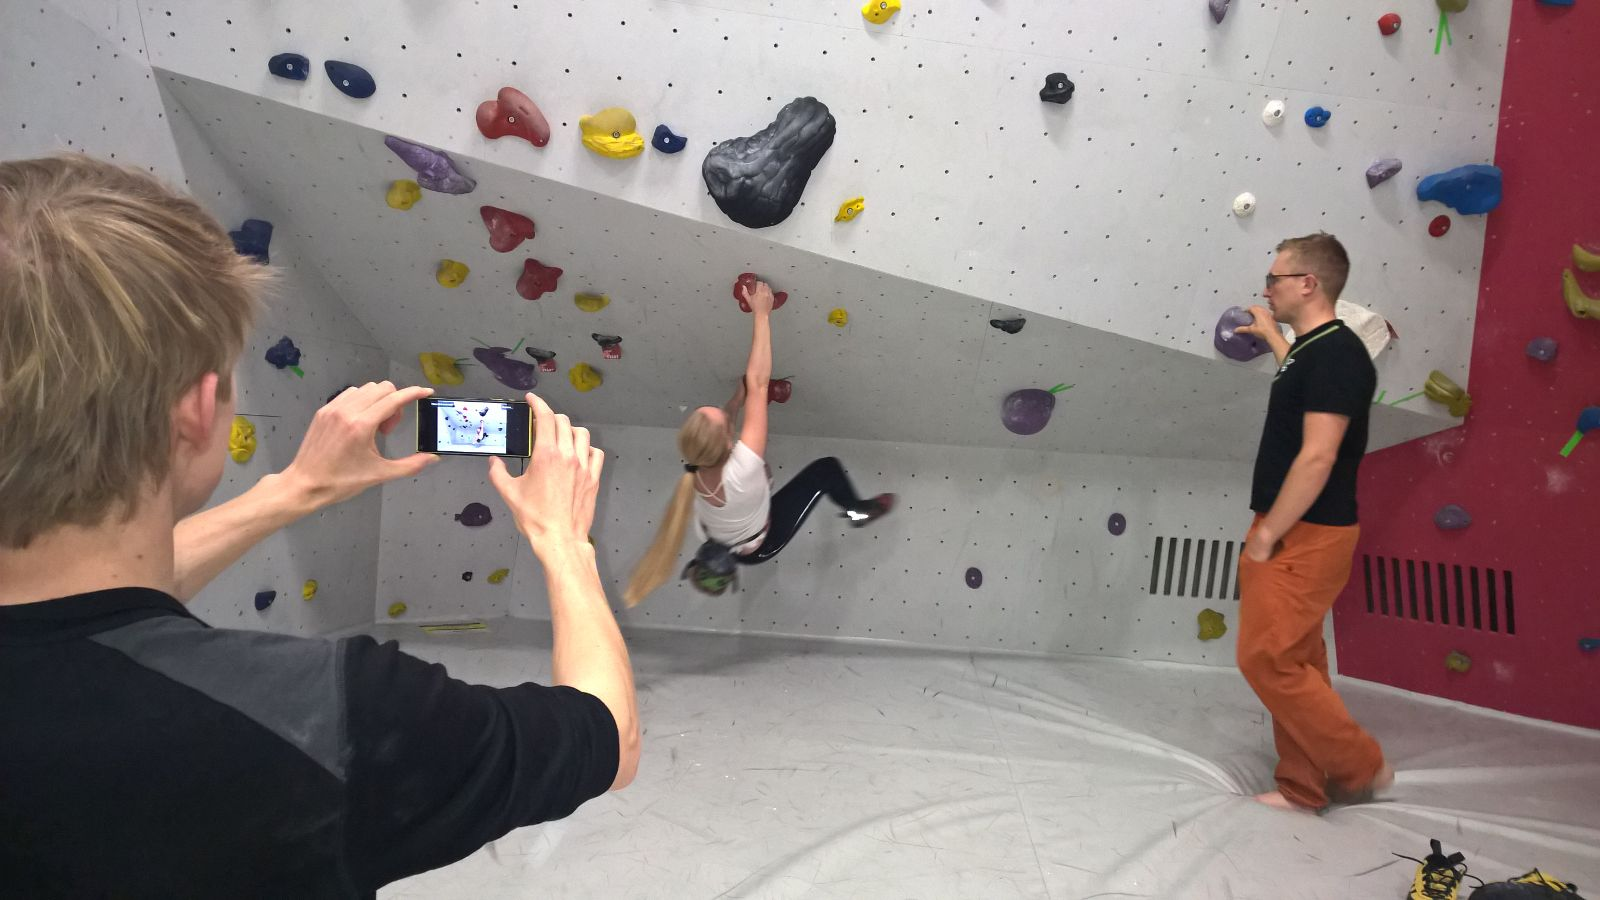
\includegraphics[width=\textwidth]{include/images/Live-Video.jpg}
		\label{fig:live-video-action}
	\end{subfigure}
	\caption{Livebildübertragung vom Smartphone (Kamera) an Google Glass Brille (Display). \\Die Kletterin kann sich selbst beim Klettern sehen, während sie klettert.}
	\label{fig:live-video}
\end{figure}
\end{frame}

\begin{frame}{Eigene Forschungsprojekte -- Crimp\textcolor{tertiary}{Bit}}
\begin{figure}[h]
	\centering
	\begin{subfigure}[t]{0.35\columnwidth}
		\centering
		\begin{overpic}[width=\textwidth]{include/images/myo-armband.jpg}
			\rbox{-9}{1}{\textcolor{source}{\tiny{Quelle: \href{https://www.myo.com}{Thalmic Labs Inc.}}}}
		\end{overpic}
		\label{fig:myo-armband}
	\end{subfigure}
	\hspace*{\fill}
	\begin{subfigure}[t]{0.62\columnwidth}
		\centering
		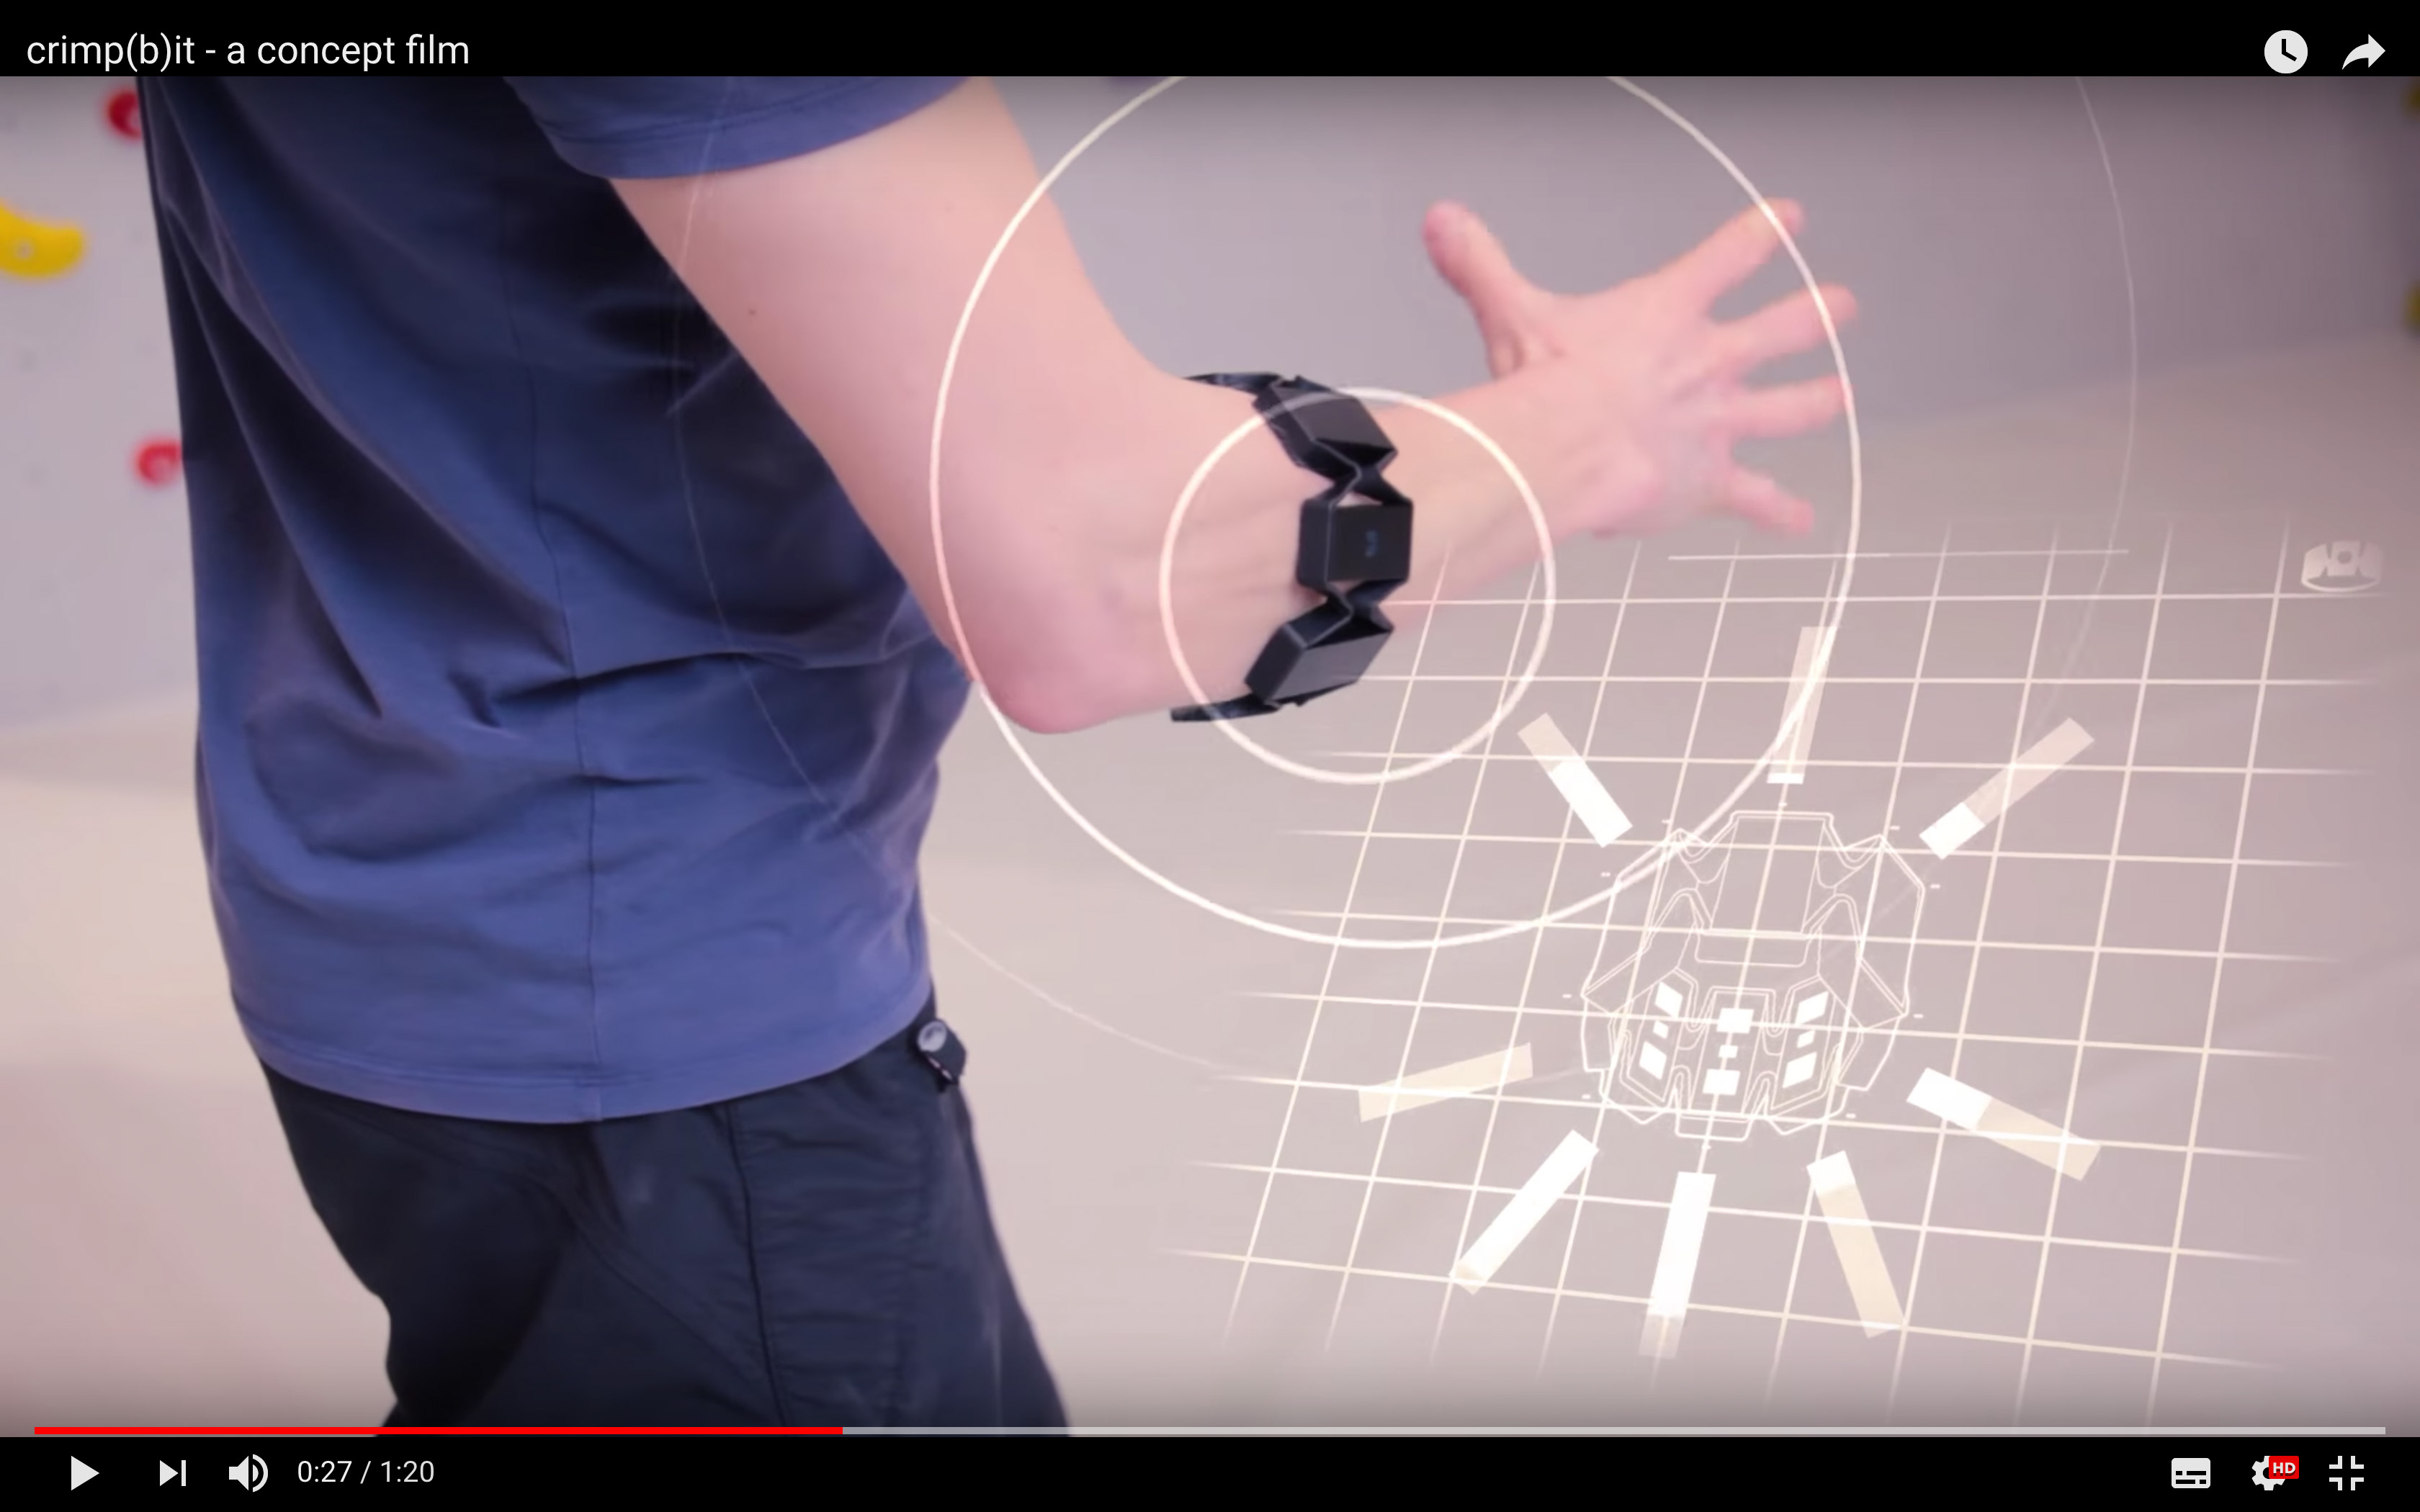
\includegraphics[width=\textwidth]{include/images/myo-demo.jpg}
		\label{fig:crimpbit-demo}
	\end{subfigure}
	\caption{MYO Armband zur Gestenerkennung als Sensor für potentiell schädliche Greifbewegungen.}
	\label{fig:crimpbit}
\end{figure}
\end{frame}

\begin{frame}{Motivation -- Grundlegende Fragestellung}
\begin{columns}
	\begin{column}{0.48\textwidth}
		\begin{itemize}[label=\textcolor{tertiary}{\faicon{caret-right}}]
			\item Forschungstrend \gls{VR}
			\item erfolgreicher Einsatz von \textit{\gls{VRET}} insbesondere \textit{bei Höhenangst} \autocite{Emmelkamp2001}
		\end{itemize}
	\end{column}
	\begin{column}{0.44\textwidth}
		\vfill
		\hfill
		\begin{overpic}[width=0.9\columnwidth]{include/images/samsung-gear-acrophobia-original.jpg}
			\rbox{-4}{1}{\textcolor{source}{\tiny{Quelle: \href{https://vrscout.com/projects/fear-of-heights-samsung-gear-vr/}{VRscout}}}}
		\end{overpic}
	\end{column}
\end{columns}
\vfill
\metroset{block=fill}
\begin{block}{Fragestellung}<2->
	Lässt sich \textcolor{tertiary}{Sturzangst}, wie auch Höhenangst, \textcolor{tertiary}{in \gls{VR} auslösen?}\\Wenn ja, welche Faktoren sind maßgebend?
	
	\hfill $\rightarrow$ Ist \gls{VR} als Trainingsmethoden denkbar?
\end{block}
\end{frame}

\begin{frame}{Studien zum Thema}
\begin{columns}
	\begin{column}{0.5\textwidth}
		\textbf{Studien zur Auswirkung von (Sturz-)Höhe beim Sportklettern}
		\autocites{Hardy2007}{Pijpers2006,Pijpers2005,Pijpers2003}
		\begin{center}
			\begin{overpic}[height=0.555\textheight]{include/images/pijpers.jpg}
				\rbox{-15}{1}{\textcolor{black}{\tiny{Quelle: \href{https://www.researchgate.net/figure/Side-view-of-the-virtual-environment-Subjects-start-in-the-Training-Room-and-later-enter_fig1_247181822}{ResearchGate}}}}
			\end{overpic}
		\end{center}
	\end{column}
	\begin{column}{0.5\textwidth}
		\textbf{Studien Auswirkung unterschiedlicher Faktoren auf das Präsenzerleben}\\
		\autocite{Meehan2002,Meehan2001}
		\begin{center}
			\begin{overpic}[height=0.53\textheight]{include/images/meehan.jpg}
				\rbox{-1}{1}{\textcolor{source}{\tiny{Quelle: \href{https://www.researchgate.net/figure/View-of-the-20-in-pit-from-the-wooden-ledge_fig3_7596875}{ResearchGate}}}}
			\end{overpic}
		\end{center}
		\vfill
	\end{column}
\end{columns}
\end{frame}

\section{Studie}

\begin{frame}{Versuchsbedingungen}
\begin{columns}
	\begin{column}{0.5\textwidth}
		\begin{enumerate}[label=\textbf\textcolor{tertiary}{\Alph*}]
			\item Reales Klettern an Griffen und Tritten
			\\\textcolor{source}{\SI{10}{\meter} über Grund}
			\item Klettern in \gls{VR} an Griffen und Tritten
			\\\textcolor{source}{visuell \SI{10}{\meter} über Grund}
			\item Klettern in \gls{VR} mit Game Controllern
			\\\textcolor{source}{visuell \SI{10}{\meter} über Grund}
		\end{enumerate}
	\end{column}
	\begin{column}{0.5\textwidth}
		\begin{center}
			\vspace*{-15mm}
			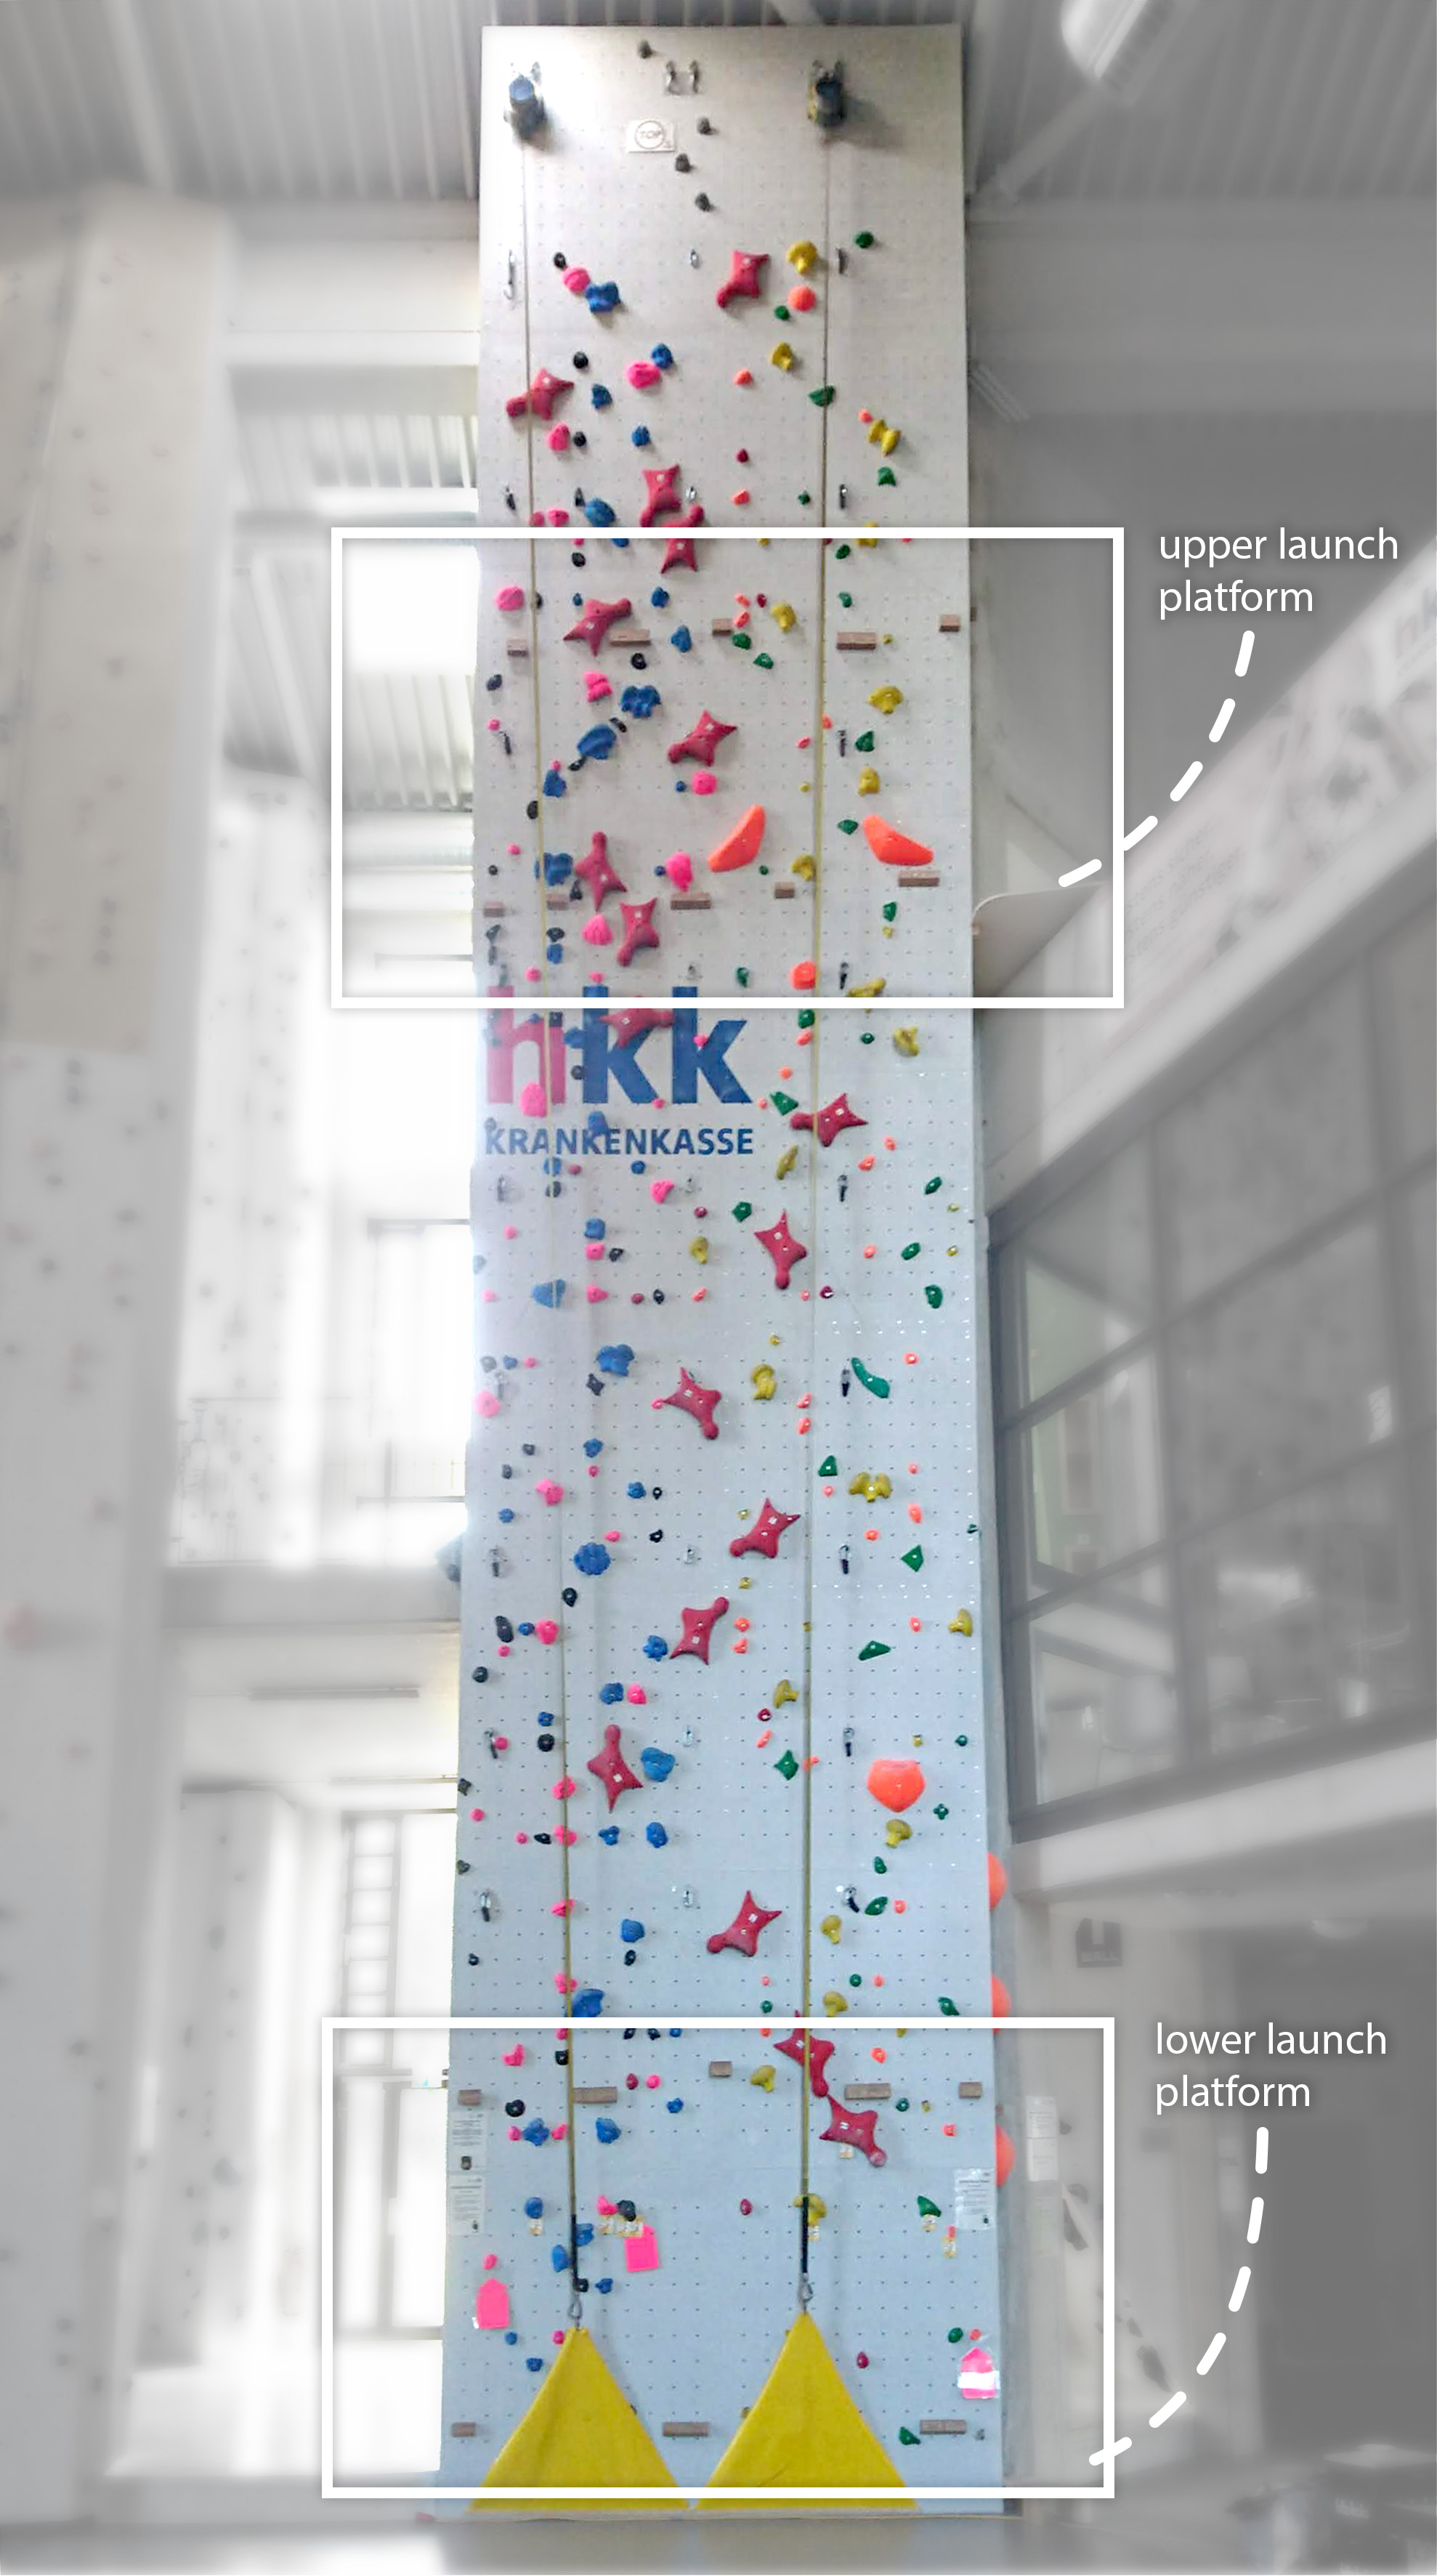
\includegraphics[height=1.2\textheight]{include/images/climbing-wall-photo.jpg}
		\end{center}
	\end{column}
\end{columns}
\end{frame}

\begin{frame}[standout]
	\begin{center}
		{\fontsize{60}{60}\faicon{youtube-play}}
	\end{center}
\end{frame}

\subsection{Technische Umsetzung}

\begin{frame}{\currentname{} -- Benötigte Komponenten}

\begin{description}
	\item[Virutal Reality System]\mbox{}
	\begin{itemize}
		\item[\textit{Kopf + Füße}] HTC VIVE
		\item[\textit{Hände}] LEAP Motion + \textbf{Unity Anbindung}
	\end{itemize}
	\item[Kletterrouten]\mbox{}
	\begin{itemize}
		\item[\textit{Real}] DAV Kletterzentrum Bremen + Eigene Griffe
		\item[\textit{Virtuell}] \textbf{3D Modell} in Maya + Unity
	\end{itemize}
	\item[Messverfahren]\mbox{}
	\begin{itemize}
		\item[\textit{Selbstauskunft}] Lime Survey Software + \textbf{Anpassung}
		\item[\textit{Biosignale}] BITalino +  wahoo TICKR X + \textbf{Android App}
	\end{itemize}
\end{description}

\end{frame}

\begin{frame}{\currentname{} -- Virtual Reality System}
	\begin{figure}
		\begin{subfigure}[t]{0.49\textwidth}
			\centering
			\begin{overpic}[width=\textwidth]{include/images/vive-kit.jpg}
				\rbox{-1}{1}{\textcolor{source}{\tiny{Quelle: \href{			https://www.inet.se/produkt/x107651/htc-vive}{HTC Corporation}}}}
			\end{overpic}
			\caption{HTC VIVE + Basistation + Controller}
		\end{subfigure}
		\begin{subfigure}[t]{0.49\textwidth}
			\centering
			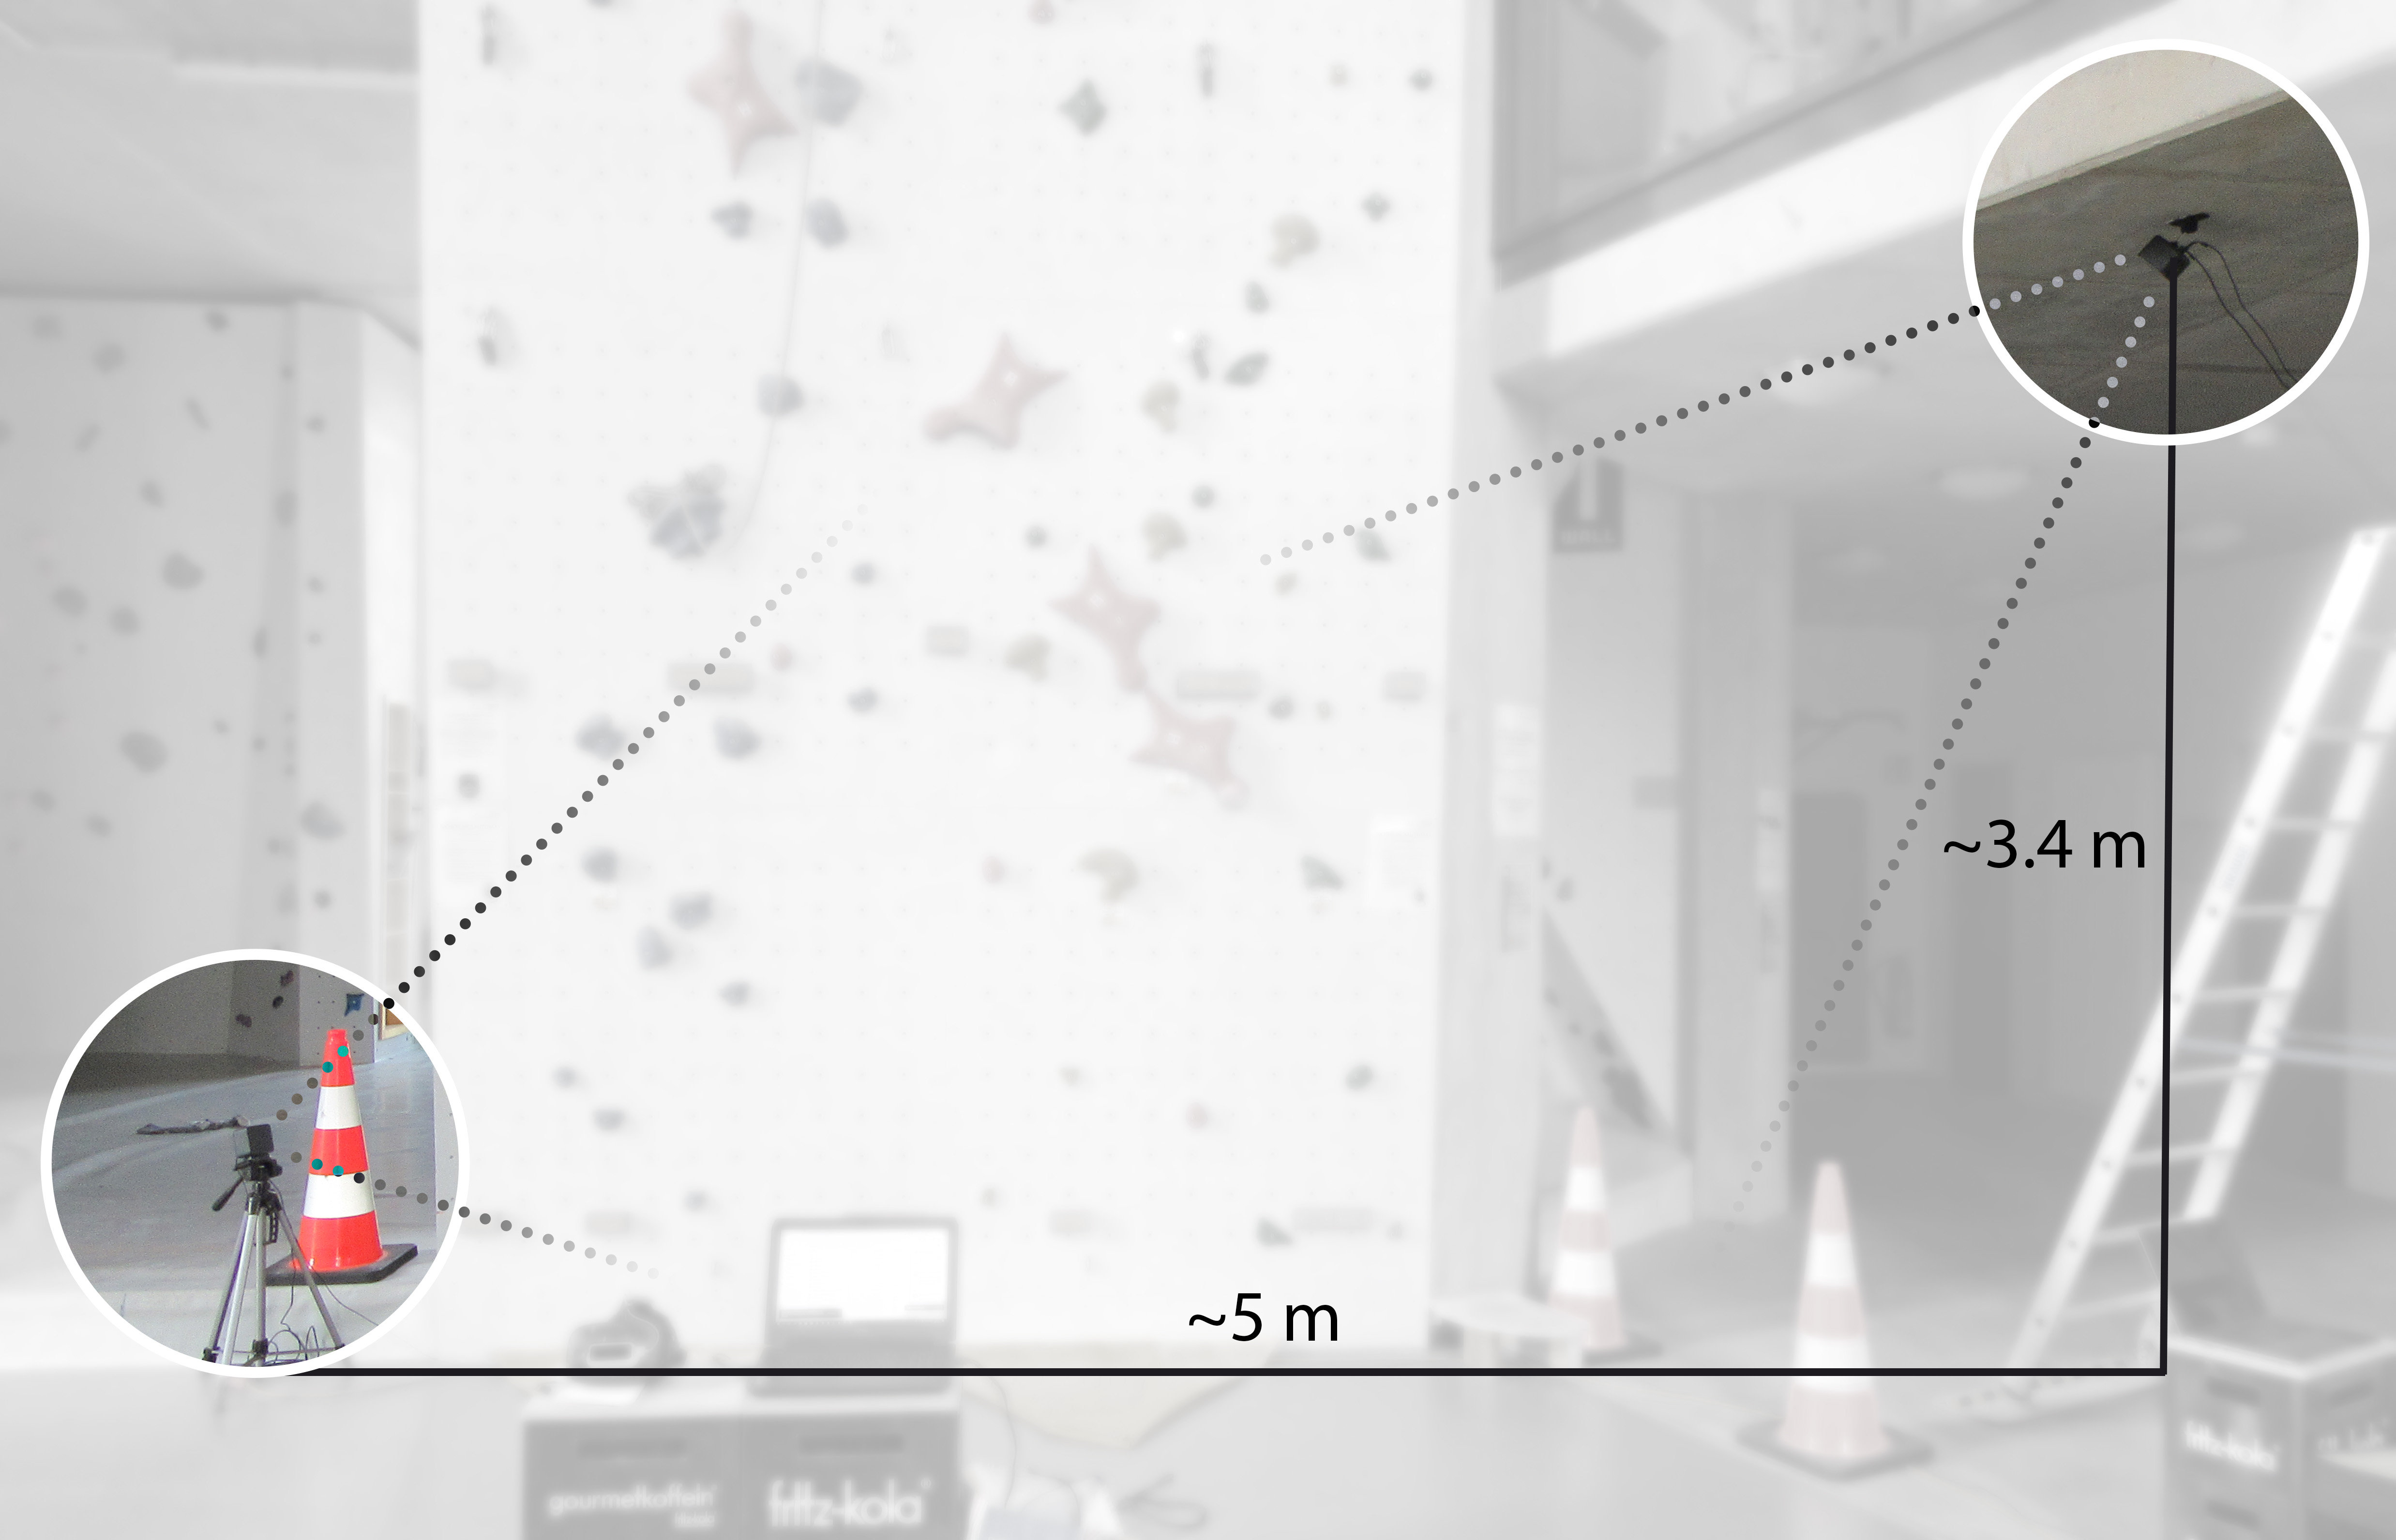
\includegraphics[width=\textwidth]{include/images/vive-setup-solution.jpg}
			\caption{HTC VIVE Position der Basistationen}
		\end{subfigure}
	\end{figure}
\end{frame}

\begin{frame}{\currentname{} -- Fuß Tracking}
\begin{figure}
	\centering
	\begin{subfigure}[t]{0.49\textwidth}
		\centering
		\includegraphics[width=\textwidth]{include/images/foot-tracking-tracker.png}
		\caption{VIVE Tracker befestigt an der Ferse}
		\label{fig:foot-tracking-tracker}
	\end{subfigure}
	\hfill
	\begin{subfigure}[t]{0.49\textwidth}  
		\centering 
		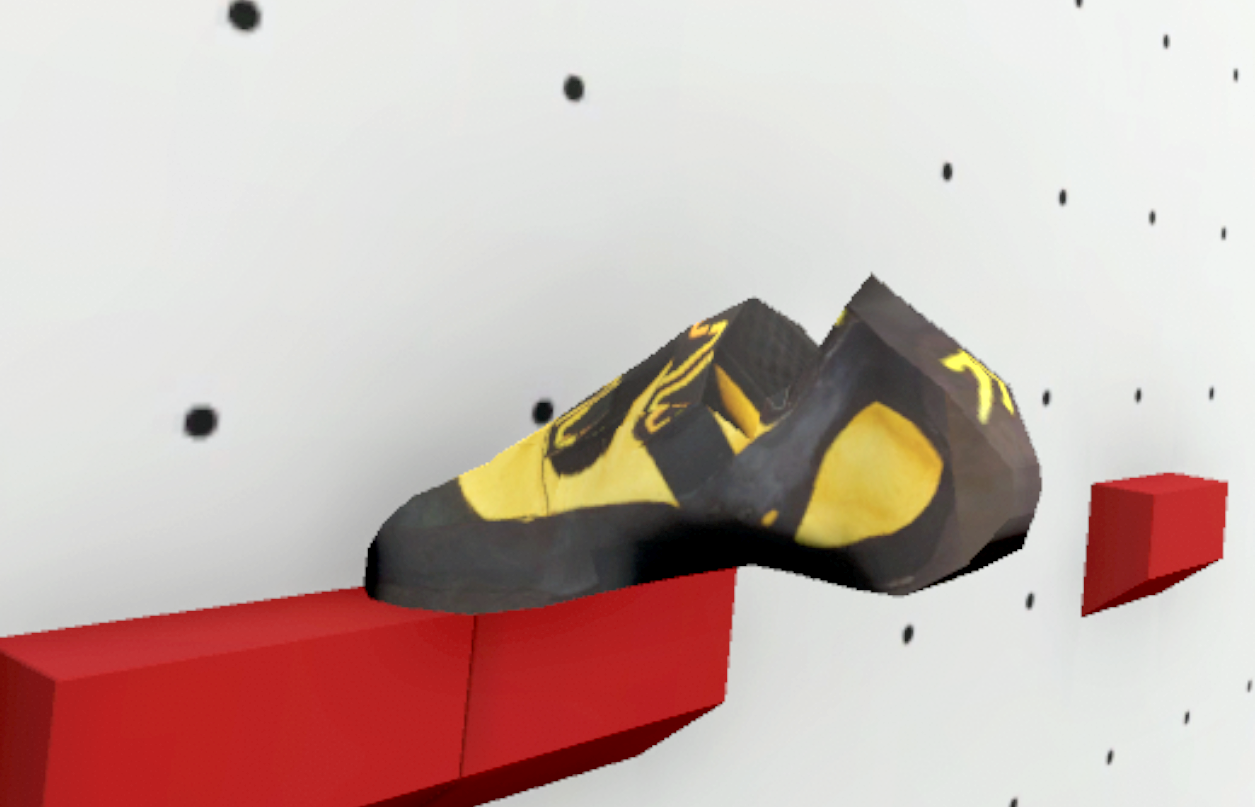
\includegraphics[width=\textwidth]{include/images/foot-tracking-result.png}
		\caption{Übertragenes Tracking auf 3D Modell in Unity}
		\label{fig:foot-tracking-result}
	\end{subfigure}
	\label{fig:foot-tracking}
\end{figure}
\end{frame}

\begin{frame}{\currentname{} -- Hand Tracking}
\begin{figure}
	\centering
	\begin{subfigure}[t]{0.32\textwidth}
		\centering
		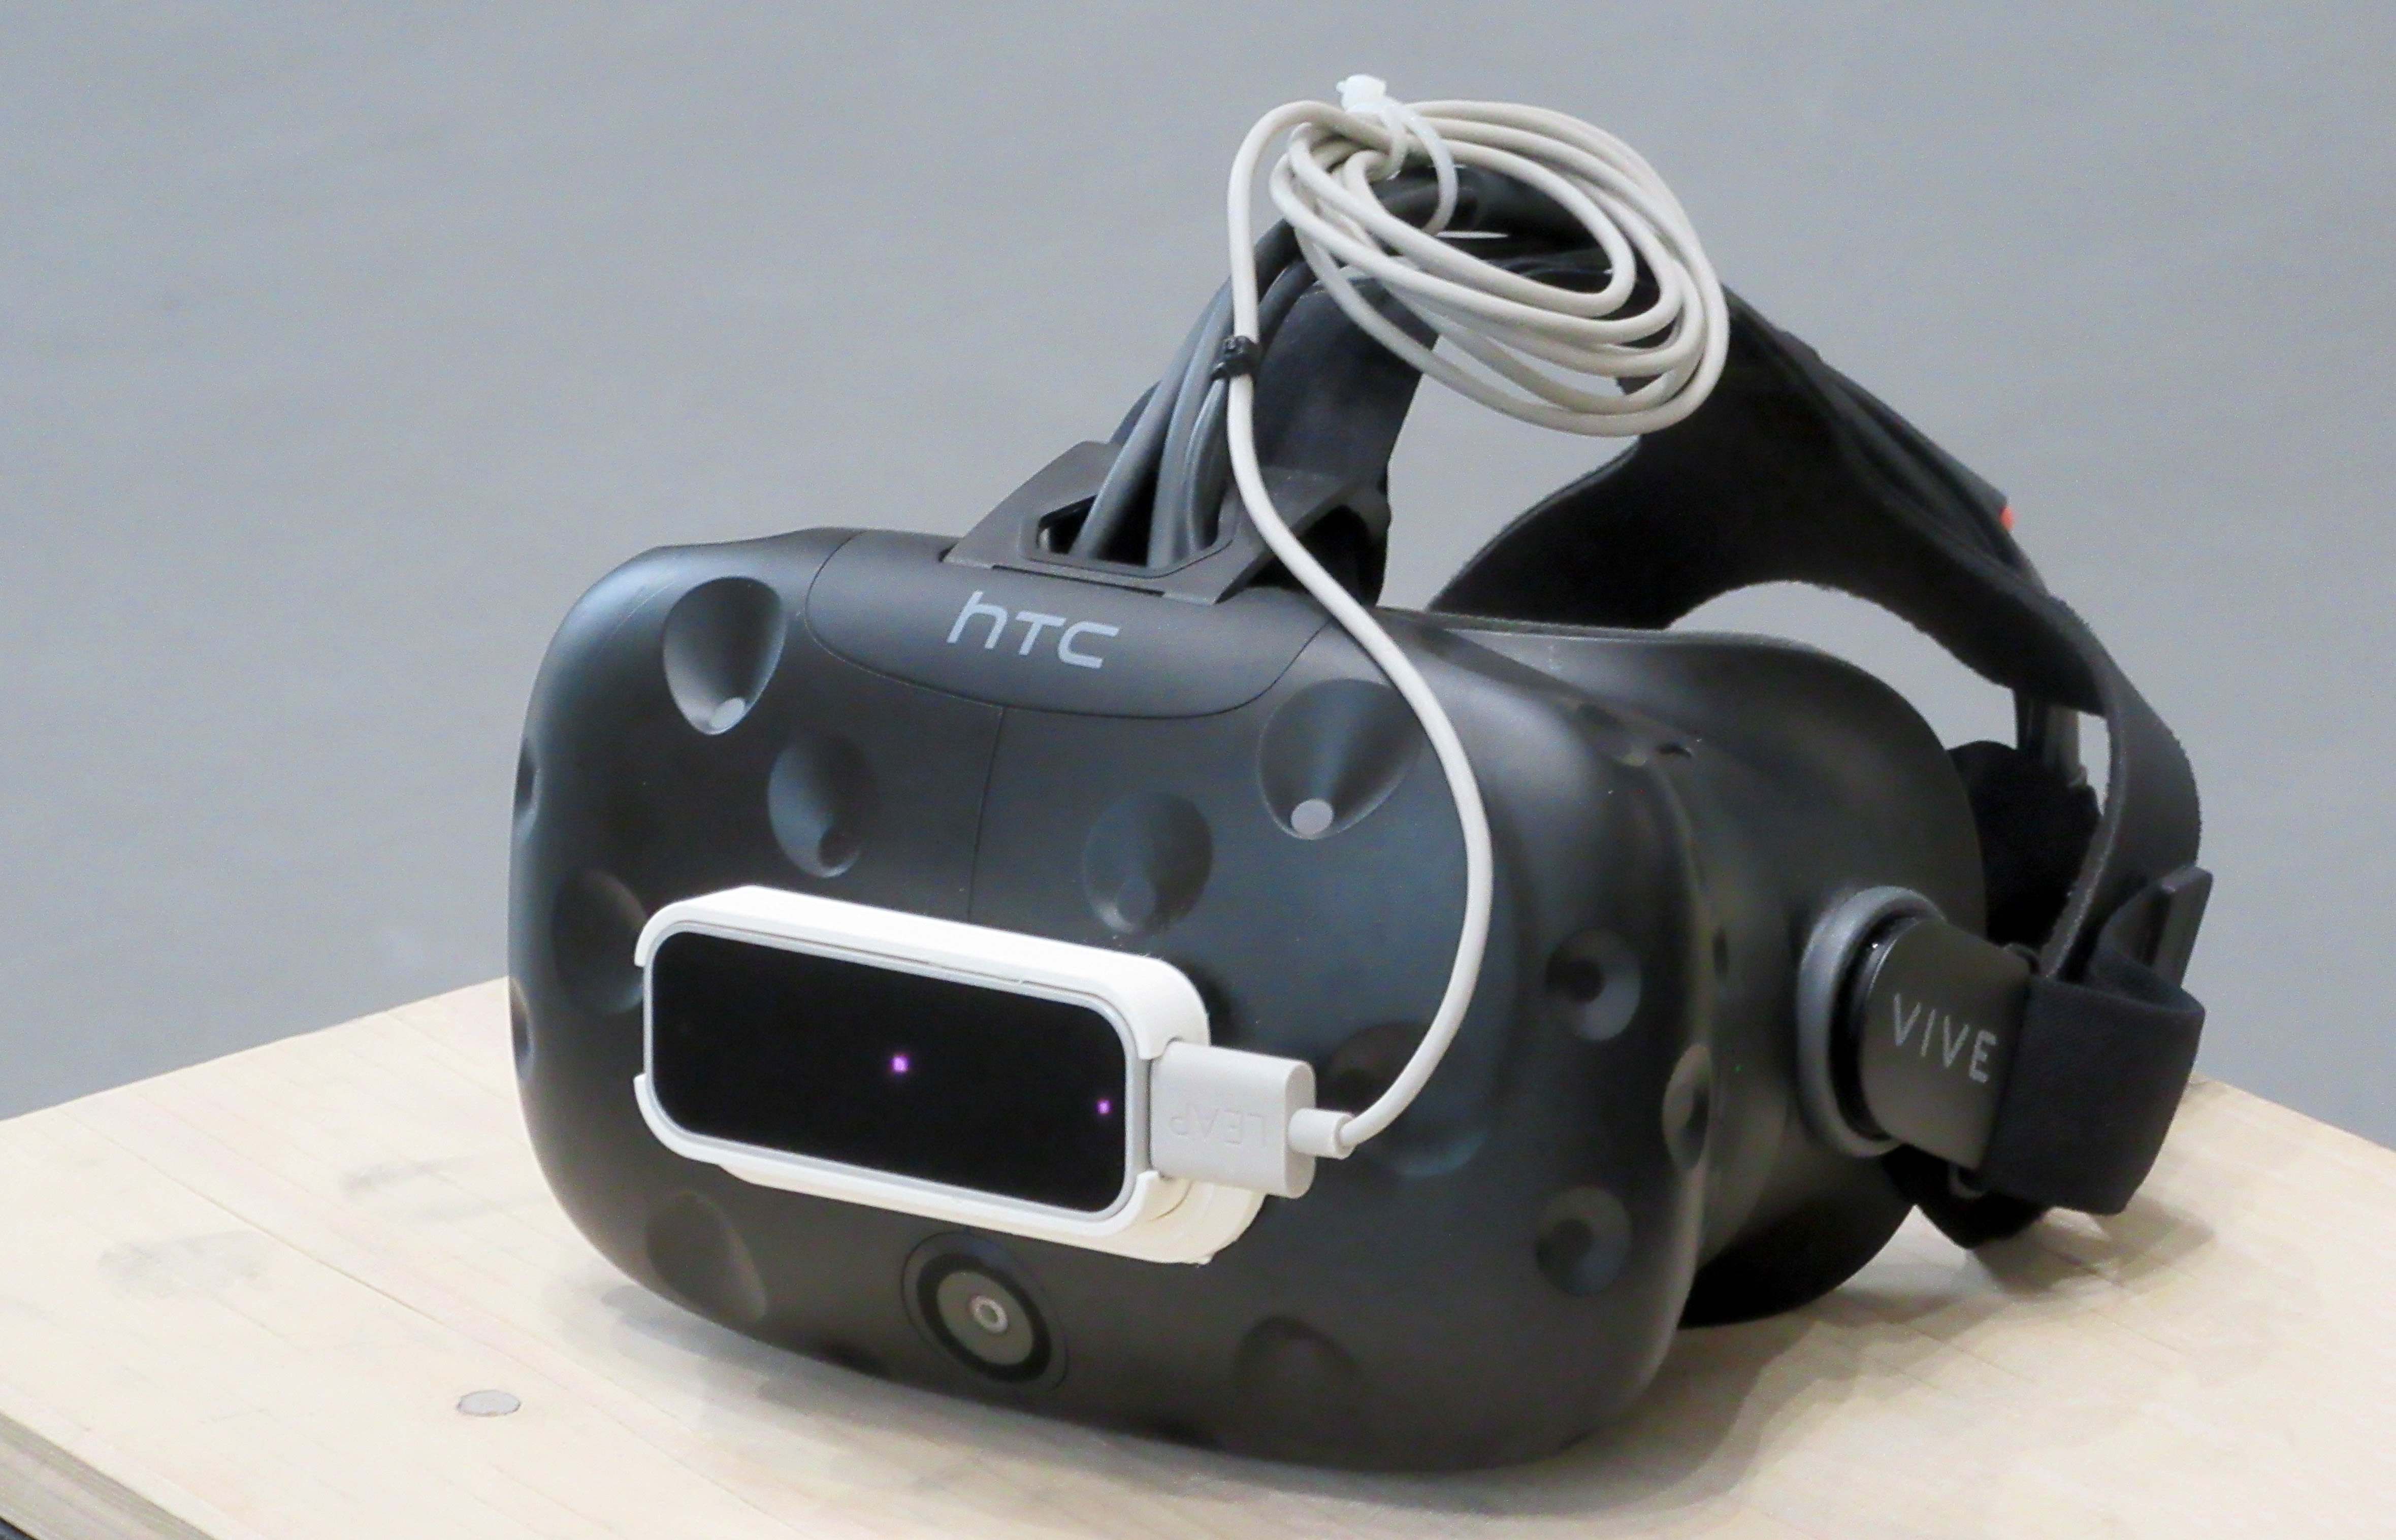
\includegraphics[width=\textwidth]{include/images/leap-motion-overlay-setup.jpg}
		\caption{LEAP Motion auf VIVE Headset}
		\label{fig:leap-motion-setup}
	\end{subfigure}
	\hfill
	\begin{subfigure}[t]{0.32\textwidth}
		\centering
		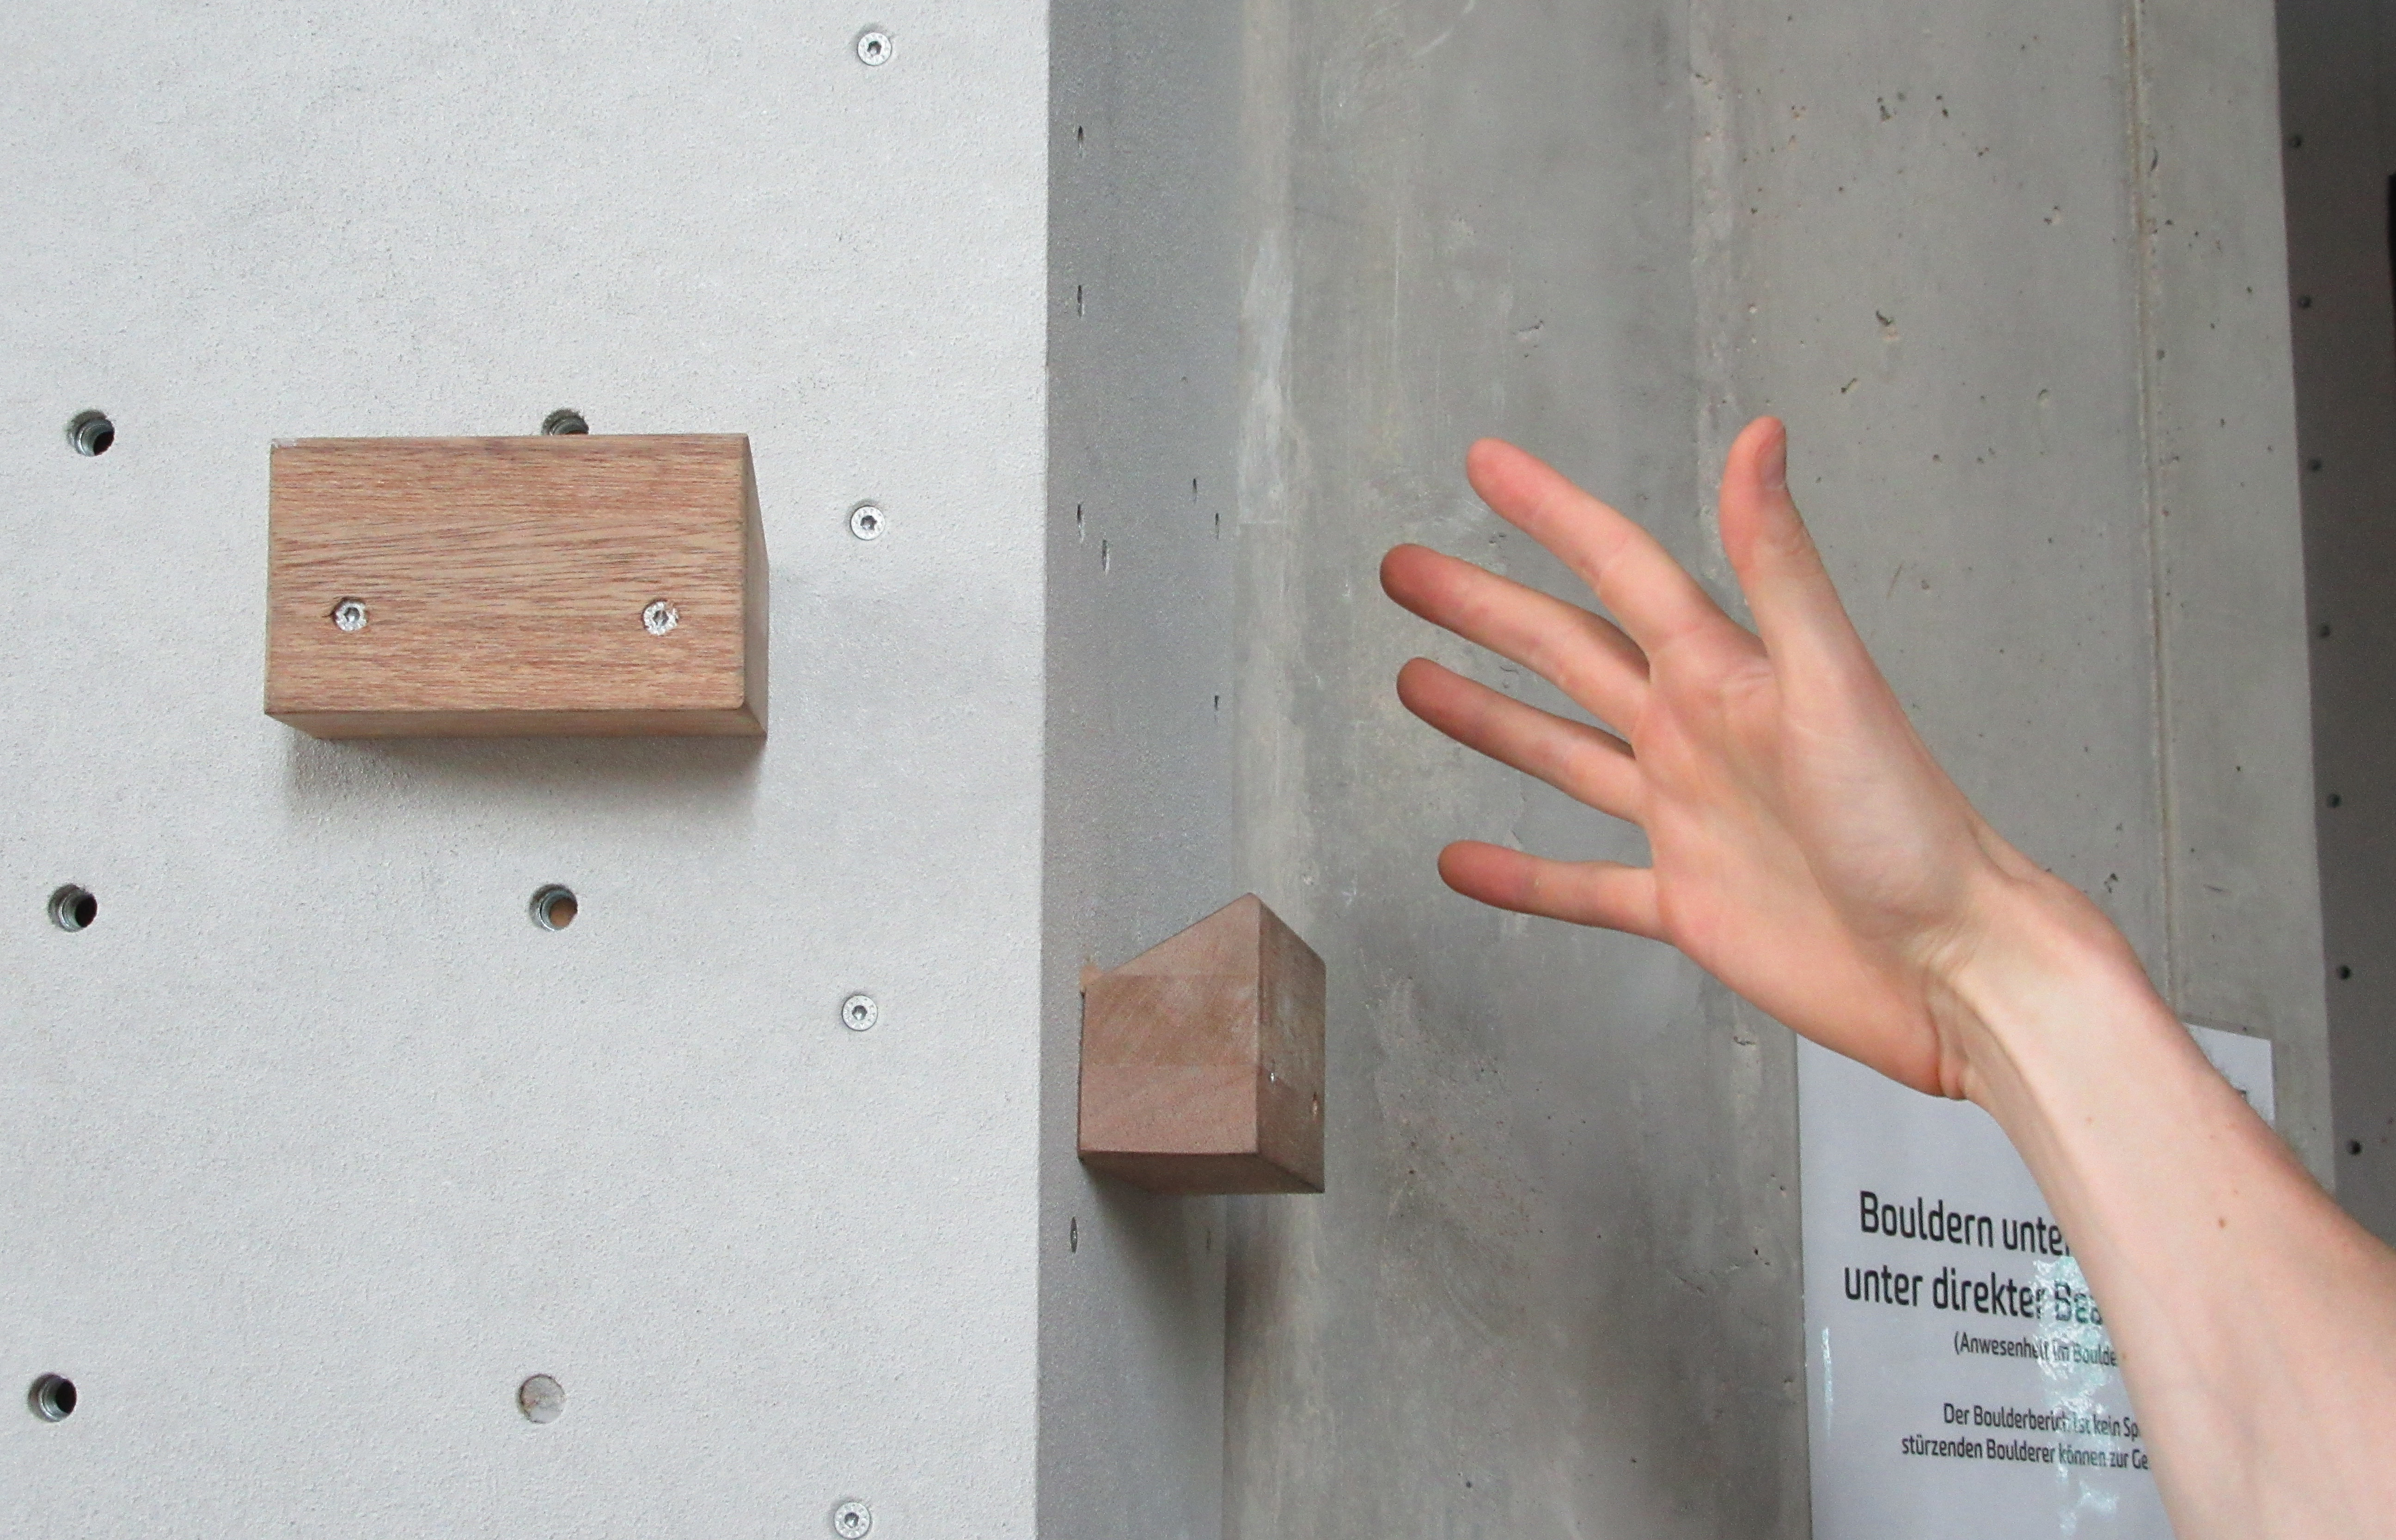
\includegraphics[width=\textwidth]{include/images/leap-motion-overlay-photo.jpg}
		\caption{Reale Perspektive (Foto)}
		\label{fig:leap-motion-overlay-photo}
	\end{subfigure}
	\hfill
	\begin{subfigure}[t]{0.32\textwidth}
		\centering
		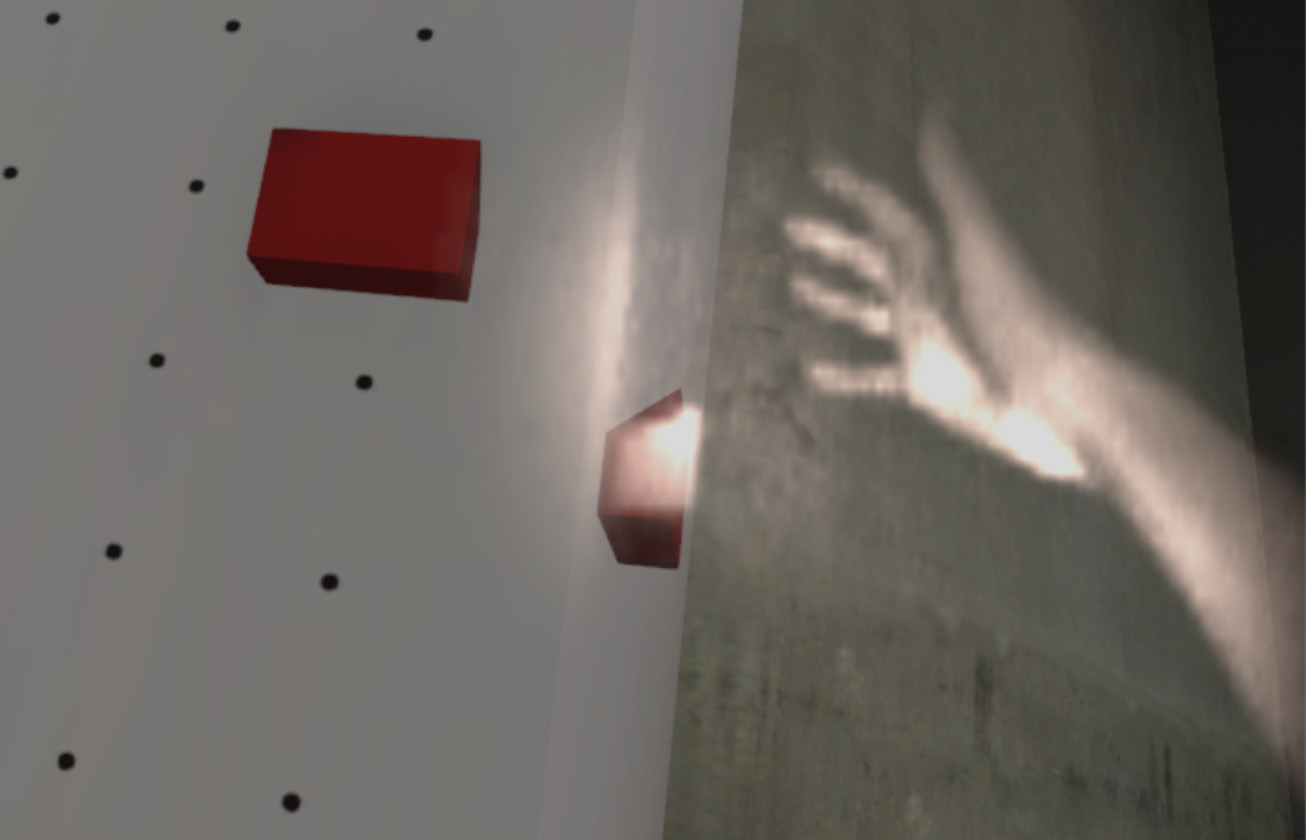
\includegraphics[width=\textwidth]{include/images/leap-motion-overlay-result.jpg}
		\caption{Resultierende des Overlays (Unity)}
		\label{fig:leap-motion-overlay-result}
	\end{subfigure}
	\captionsetup{subrefformat=parens}
	\caption[Leap Motion hand tracking]{Hand Overlay erzeugt aus einem Infrarotbild des LEAP Motion Sensors \subref{fig:leap-motion-setup} welches weich anhand des 3D Modells maskiert wird $\rightarrow$ nahegelegene Griffe bleiben sichtbar \subref{fig:leap-motion-overlay-result}}
	\label{fig:leap-motion-overlay}
\end{figure}
\end{frame}

\begin{frame}{\currentname{} -- Biosignalerfassung}
\begin{figure}
	\centering
	\begin{subfigure}[b]{0.49\textwidth}
		\centering
		{
			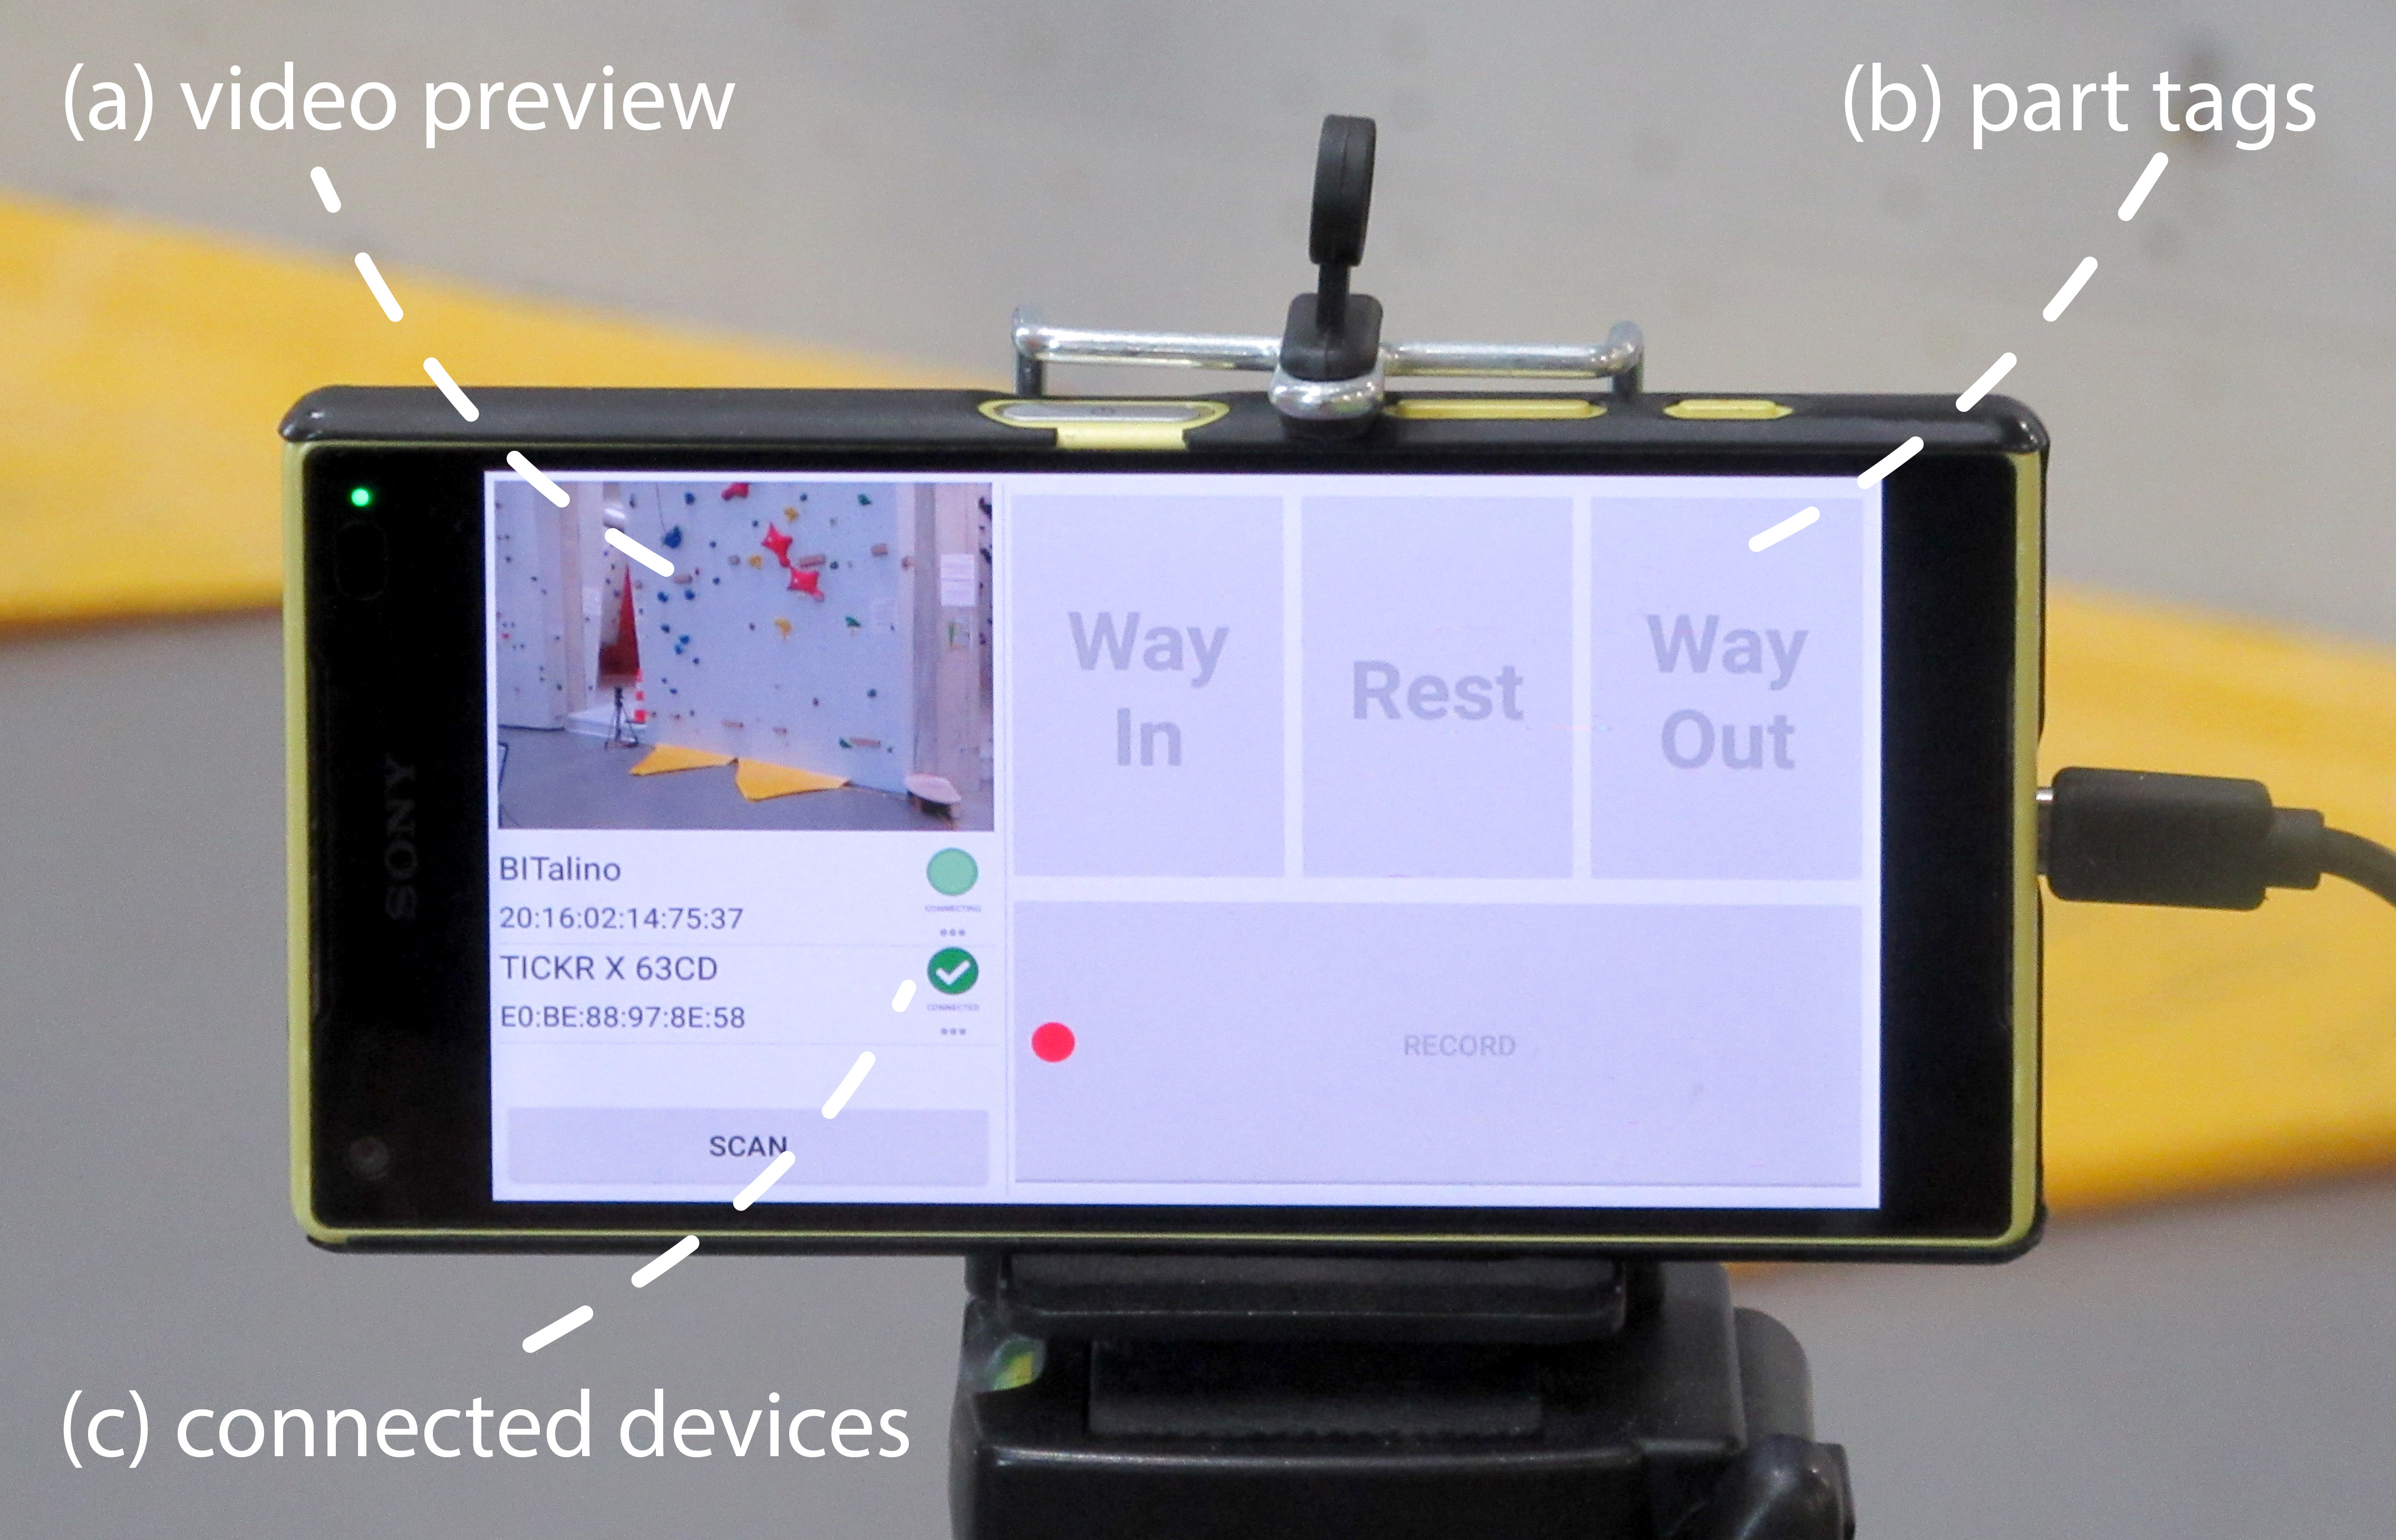
\includegraphics[width=\textwidth]{include/images/android-app-photo.jpg}
			\phantomsubcaption\label{fig:android-app-preview}
			\phantomsubcaption\label{fig:android-app-parts}
			\phantomsubcaption\label{fig:android-app-devices}
		}
		\captionsetup{subrefformat=parens}
		\caption{Android App zur Erfassung der Biosignale, mit Videovorschau \subref{fig:android-app-preview}, einer Liste verbundener Sensoren \subref{fig:android-app-devices} und Knöpfen zum Markieren der Versuchsabschnitte \subref{fig:android-app-parts}}
		\label{fig:android-app}
	\end{subfigure}
	\hfill
	\begin{subfigure}[b]{0.49\textwidth}  
		\centering
		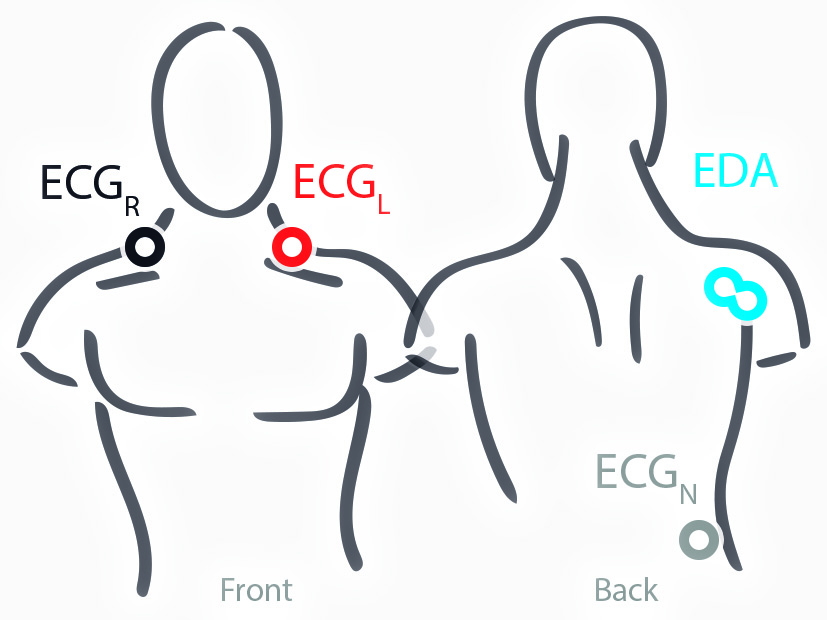
\includegraphics[width=\textwidth]{include/images/electrodes.jpg}
		\caption{Schematische Übersicht zur Platzierung Elektroden für ECG (Herzschlag) und EDA (Hautleitfähigkeit) in Anlehnung an \textcite{ECGLeadPlacement2015}}
		\label{fig:electrodes-schema}
	\end{subfigure}
	\label{fig:biosignals}
\end{figure}
\end{frame}

\subsection{Methode}

\begin{frame}[standout]
\begin{center}
			\parbox{0cm}{%
		\LARGE
		\begin{tabbing}
			\faicon{check-square} \quad \= Technische Umsetzung\\
			\faicon{square} \> Studiendurchführung
		\end{tabbing}}
\end{center}
\end{frame}

\begin{frame}{\currentname{} -- Ablauf}
	\begin{enumerate}[label=\textbf\textcolor{tertiary}{\theenumi}]
		\item Belehrung, Gurt anlegen, Elektroden anlegen
		\item Vorabfragebogen zum allgemeinen Befinden (STAI-T)
		\item Durchlaufen der Bedingungen A, B und C (randomisiert nach Latin Square)
		\\Fragebögen im Anschluss an
		\begin{itemize}
			\item[\textit{A}] \gls{RPE} und \gls{AT}
			\item[\textit{B, C}] \gls{IPQ}, \gls{RPE} und \gls{AT}
		\end{itemize}
		\item kurzes, mündliches Interview
	\end{enumerate}
\end{frame}

\subsection{Ergebnisse}

\begin{frame}{\currentname{} -- Teilnehmer*innen}
	\begin{itemize}[label=\textcolor{tertiary}{\faicon{caret-right}}]
		\item 28 (13 w, 15 m) Teilnehmer*innen, 
		\item Alter: 30,7 Jahre (SD = 10.6)
		\item Können: Vorstieg (23), 6+ (± 1 Grad); Top-Rope (5), 5+/6- (±1 Grad) \textcolor{source}{Skala: UIAA}
		\item VR Vorerfahrung: keine (13), minimal (13), selten (2)
		\item keine überdurchschnittliche Ängstlichkeit (nach STAI-T)
		\item keine klinische Höhenangst (nach vHI)
	\end{itemize}
\end{frame}

\begin{frame}{\currentname{} -- Vergleichbarkeit}
\begin{tabbing}
	\textcolor{primary}{\faicon{question-circle}} \quad \= Welchen Effekt hat die Bedingung (Griffe/Tritte|Controller) auf Präsenz/Angst?
\end{tabbing}
	\only<2->{\begin{figure}[htb]
	\centering
	\begin{subfigure}[t]{0.49\columnwidth}
		\centering
		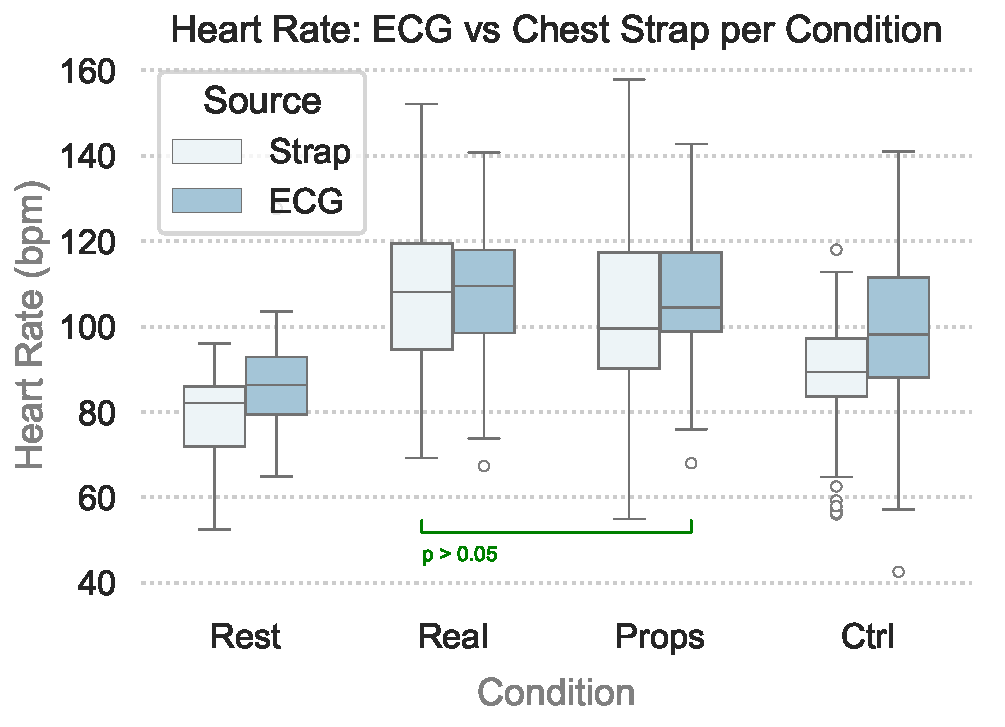
\includegraphics[width=\textwidth]{include/images/hr_per_condition_by_source.pdf}
		\label{fig:physical-exertion-hr}
	\end{subfigure}
	\hspace*{\fill}
	\begin{subfigure}[t]{0.49\columnwidth}
		\centering
		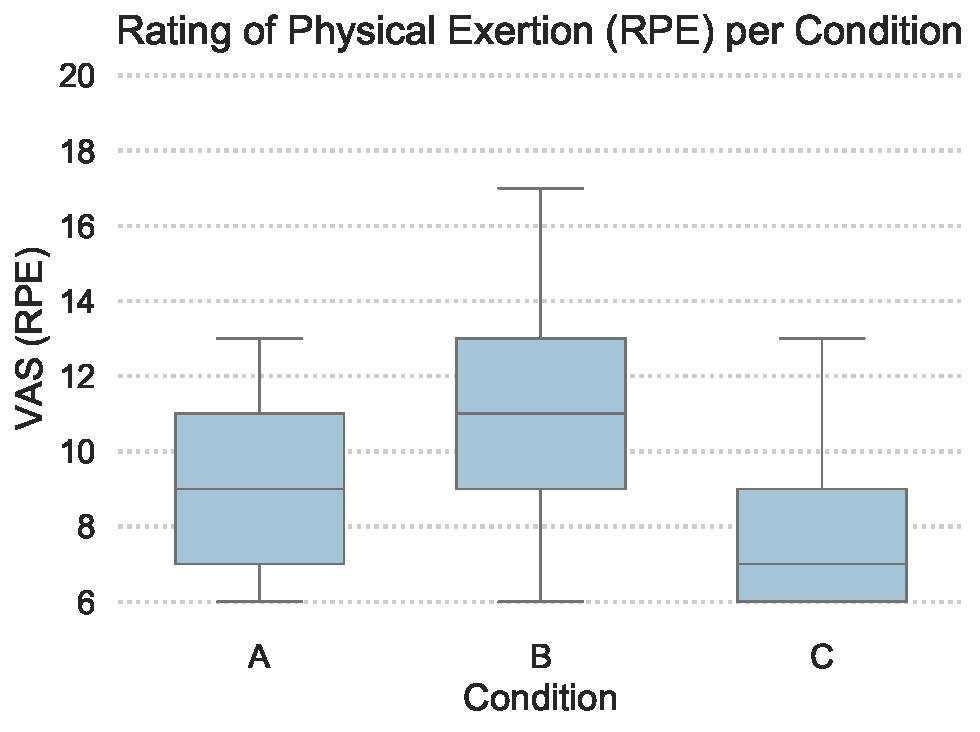
\includegraphics[width=\textwidth]{include/images/rpe_per_condition.pdf}
		\label{fig:physical-exertion-rpe}
	\end{subfigure}
	\label{fig:physical-exertion}
\end{figure}}
\end{frame}

\begin{frame}{\currentname{} -- Angst}
\begin{figure}[htb]
	\centering
	\begin{subfigure}[t]{0.49\columnwidth}
		\centering
		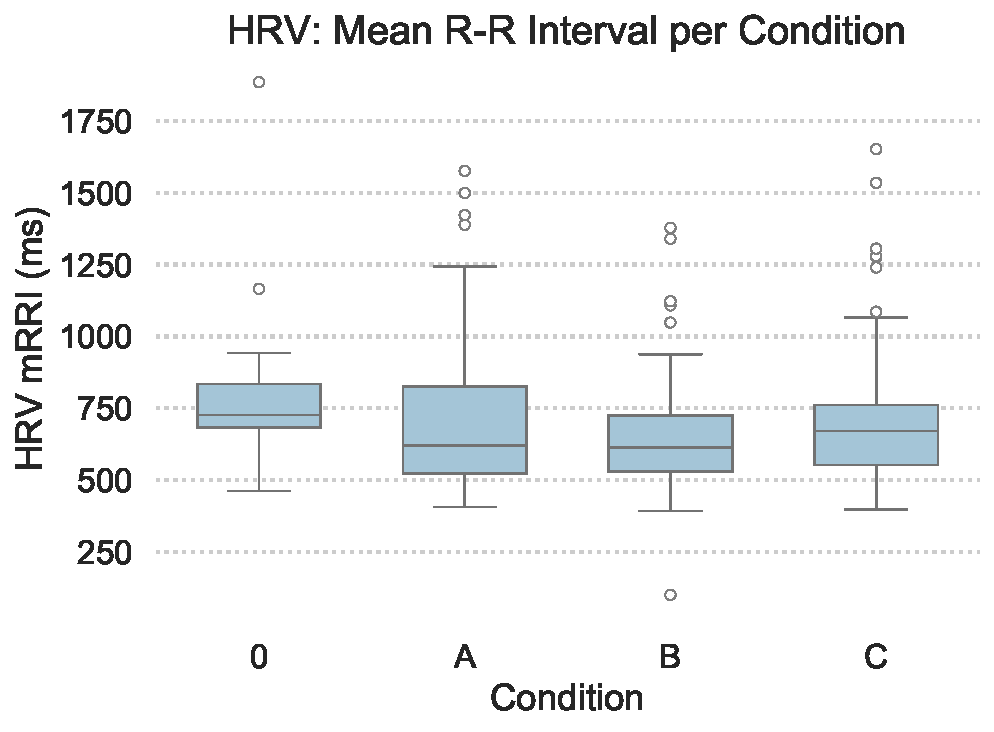
\includegraphics[width=\textwidth]{include/images/hrv_per_condition.pdf}
		\label{fig:stress-hrv}
	\end{subfigure}
	\hspace*{\fill}
	\begin{subfigure}[t]{0.49\columnwidth}
		\centering
		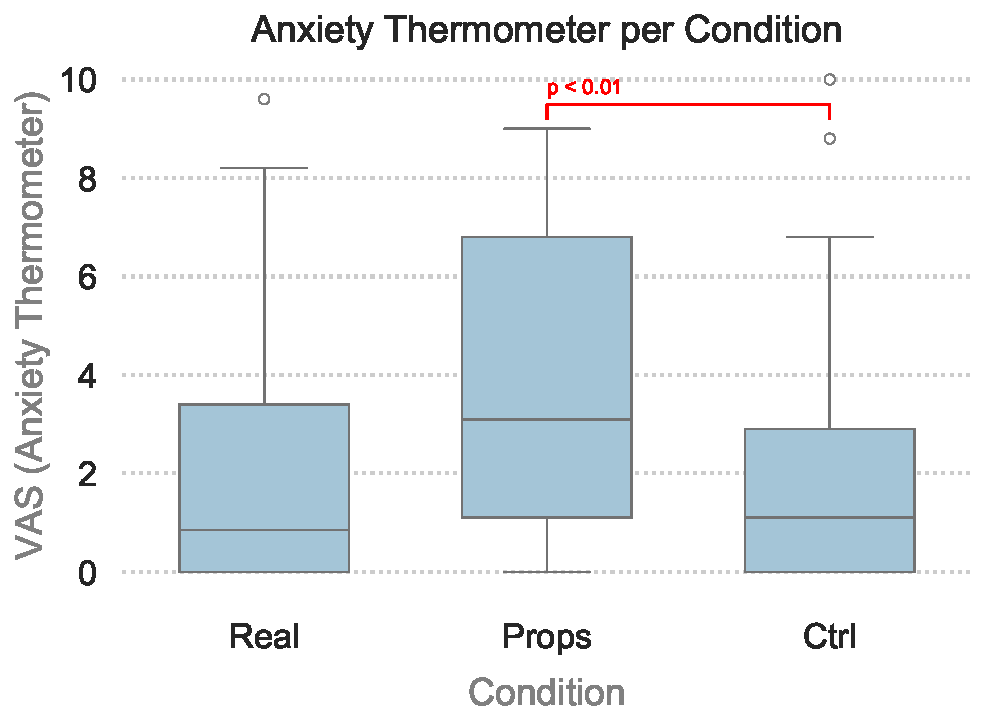
\includegraphics[width=\textwidth]{include/images/at_per_condition.pdf}
		\label{fig:anxiety-at}
	\end{subfigure}
	\label{fig:stress-anxiety}
\end{figure}
\end{frame}

\begin{frame}{\currentname{} -- Präsenz}
\begin{figure}[htb]
   \begin{center}
   	   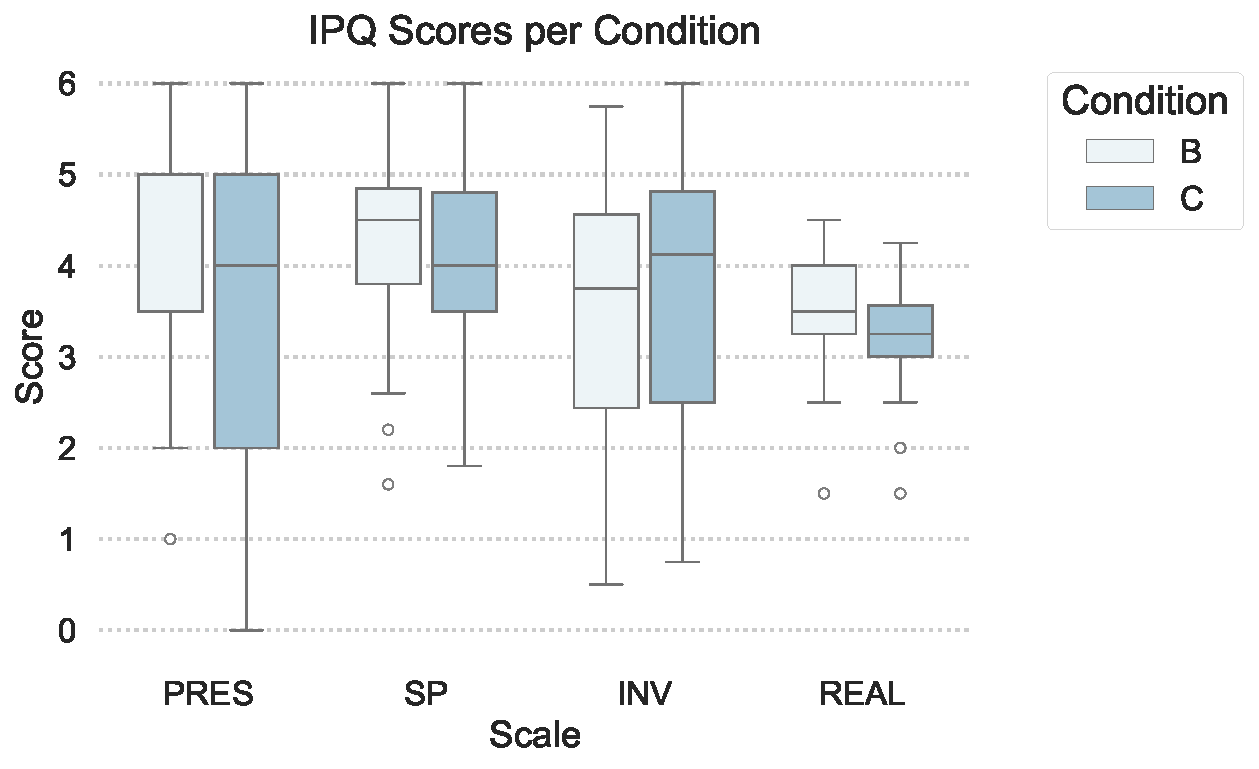
\includegraphics[width=0.6\textwidth]{include/images/ipq_per_condition}
   	\captionsetup{subrefformat=parens}
   	\caption{\gls{IPQ} Werte für die Bedingungen B und C auf den Skalen \textit{general presence} (PRES), \textit{spatial awareness} (SP), \textit{involvement} (INV), and \textcolor{secondary}{\textit{realness} (REAL)}}
   	\label{fig:presence}
   \end{center}
\end{figure}
\end{frame}

\subsection{Diskussion}

\begin{frame}{\currentname{} -- Mehrdeutigkeit}
\begin{tabbing}
	\textcolor{primary}{\faicon{question-circle}} \quad \= Welchen Effekt hat die Bedingung (Griffe/Tritte|Controller) auf Präsenz/Angst?
\end{tabbing}
\begin{description}
	\item[Präsenz/Angst]\mbox{}
	\begin{itemize}
		\item[\textit{Psych.}] Griffe/Tritte $\rightarrow$ \textbf{erhöhte} Präsenz u. Angst
		\item[\textit{Phys.}] \textbf{kein Unterschied} messbar zw. Griffe/Tritte|Controller
	\end{itemize}
\end{description}
\end{frame}

\begin{frame}{\currentname{} -- Welche Angst?}
\begin{description}
	\item[Selbstwahrnehmung]\mbox{}
	\begin{itemize}[label=\textcolor{tertiary}{\faicon{caret-right}}]
		\item Auslöser unklar, nicht zwingend Sturzangst
		\item Alternativer Ursprung: Unsicherheit mit VR System
	\end{itemize}
	\item[Biosignale]\mbox{}
	\begin{itemize}[label=\textcolor{tertiary}{\faicon{caret-right}}]
		\item Hautleitfähigkeit zeigt keine konsistente Veränderung
		\item Vermutung: Durchschnittswerte unpassend; Bewegungsartefakte
	\end{itemize}
\end{description}
\end{frame}

\section{Fazit und Ausblick}

\begin{frame}{\currentname{}}
	\textbf{Höhen-, Flug-, \textcolor{secondary}{und Sturzangst?}}
	\begin{itemize}[label=\textcolor{tertiary}{\faicon{caret-right}}]
		\item Ja und nein $\rightarrow$ mehr Forschung nötig zu Angst + physische Aktivität
	\end{itemize}
	\textbf{Technologischer Mehrwert}
	\begin{itemize}[label=\textcolor{tertiary}{\faicon{caret-right}}]
		\item neuartige, präzise Darstellung von Händen in VR zur physischen Interaktion
	\end{itemize}
	\vfill{}
	\hfill{}\textit{VR \xcancel{Therapie} Training für Sturzangst bleibt Zukunftsmusik} \textcolor{secondary}{\faicon{sign-out}}
\end{frame}

\begin{frame}[plain]
\begin{center}
	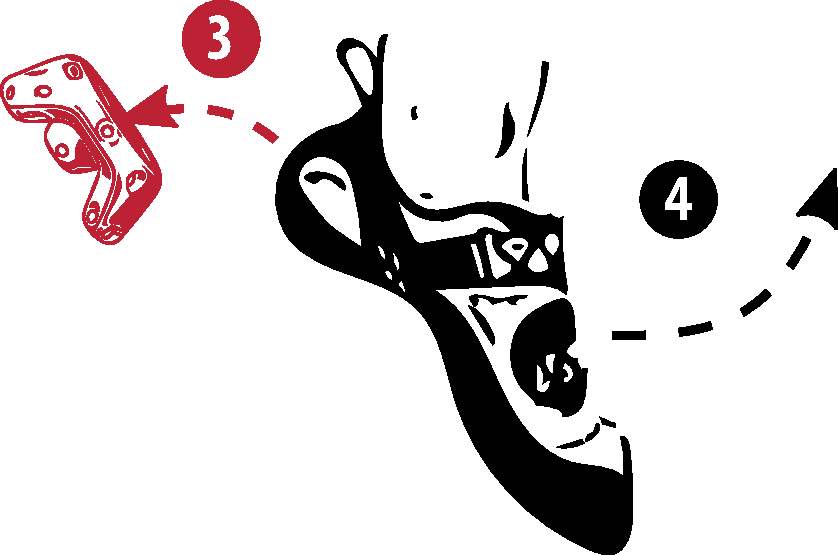
\includegraphics[width=0.8\textwidth]{include/images/climbing-shoe-with-instructions-off.pdf}
\end{center}
\end{frame}
